\documentclass[12pt, a4paper]{report}
\usepackage[utf8]{inputenc}
%subpackage
\usepackage{subcaption}
\usepackage{float}
% hyperref
\usepackage[bookmarks, colorlinks, breaklinks]{hyperref}  % PDF hyperlinks, with coloured links
\hypersetup{linkcolor=black, citecolor=black, filecolor=black, urlcolor=black} % black links, for printed output

% Support for the inclusion of figures
\usepackage{graphicx}

% "Contents" and "bibliography" are included in the summary.
\usepackage{tocbibind}

% Packages and configuration for Alloy code listing
%\usepackage{listings}
%\usepackage{alloy}
%\usepackage{color}
%\definecolor{alloy-keyword}{rgb}{0.23, 0.23, 0.7}
%\definecolor{alloy-comment}{rgb}{0.18, 0.64, 0.18}
%\definecolor{alloy-string}{rgb}{0.71, 0.18, 0.71}

\def\chapterautorefname{Chapter}

\begin{document}
<<<<<<< HEAD
\title{Software Engineering 2: TrackMe \\ \vspace{1em} Design Document}
\author{Haritha Harikumar, Mohini Gupta, Saloni Kyal\\
Politecnico di Milano}
\date{December 10, 2018}
=======
\title{Software Engineering 2: TrackMe \\ \vspace{1em} Requirements Analysis and Specification Document}
\author{Haritha Harikumar, Mohini Gupta, Saloni Kyal\\
Politecnico di Milano}
\date{November 11, 2018}
>>>>>>> c41ec8f0b0b1545b1fda6c11f51fbdc5631db9e7
\maketitle
\tableofcontents

%%%%%% INTRODUCTION %%%%%%%%
\chapter{Introduction}
\label{ch:introduction}

\section{Purpose}
<<<<<<< HEAD
TrackMe is an android application developed by TrackMe. The application helps to monitor health vitals and location of individuals. TrackMe stands apart from other health monitoring application with its features that enables 3rd party services to monitor the data of individuals for a valid cause. TrackMe also provides other useful services like emergency alerts to ambulances in case an individual's vitals are in critical condition. Apart from that TrackMe comes with a service which offers people or a group of people to organize and visualize races or marathons. 

This following document focuses on describing TrackMe system with respect to its goals and requirements and then formulating the functional and non-functional requirements. The document also provides an ample idea of the process flow and a model of the application with the help of  diagrams and mock-ups.

Further, this document will provide formal specification of some features of the applications, by means of the Alloy language~\cite{alloy-site}.

=======
<<<<<<< HEAD
TrackMe is an android application developed by TrackMe. The application helps to monitor health vitals and location of individuals. TrackMe stands apart from other health monitoring application with its features that enables 3rd party services to monitor the data of individuals for a valid cause. TrackMe also provides other useful services like emergency alerts to ambulances in case an individual's vitals are in critical condition. Apart from that TrackMe comes with a service which offers people or a group of people to organise and visualise races or marathons. 

This document is intended to be examined by a group of developers that will implement our system to make the implementation consistent with the system project.



\section{Scope}
\qquad Track4Me is a company which provides three software based services. The services are limited to the citizens of Milan. The given problem is to design and develop a software service called  “Data4Help”,  which acts as an intermediary between the individuals and the other companies. It targets two set of users, individuals and third party. The location and health of the user is extracted from a wearable device. The data from the wearable device is extracted with the help of the API of the wearable device. The software tracks the location and health status of individuals or group of individuals and send the information to the third party on their request to monitor the health of individuals by validating the type of requests. The validation of the requests for the information of specific individuals is done by the individual’s self acceptance or rejection. The requests for the information of group of individuals is decided by Track4Me and generalized by allowing the access to the third party, if the number of individuals whose information is to be accessed is greater than 1000.

\qquad It builds a new service called “AutomatedSOS” over the top of “Data4Help” after monitoring the demand of requests from third parties for giving non-intrusive SOS service to elderly people, which sends the ambulance to individual’s location when the health parameters are below the thresholds. The nearest ambulance is tracked and sent to ensure individual’s quick and efficient recovery. A separate mobile application of Track4Me is to be exclusively developed for the ambulance drivers who are informed by push notifications in the mobile application along with the location and other details of the patient in less than 5 seconds to ensure spontaneity in reaction to emergencies. All the hospitals in Milan are informed to ensure all the ambulance drivers installs TrackMe application.

\qquad A new service called “Track4Run” is built as a source of revenue which allows organizer to organize an event, athletes to participate in the event and spectators to see the athletes position live in a Map. It exploits the service of “Data4Help” which tracks the location of the athletes to be visible to everyone and helps the organizer to monitor the health status of athletes as well. The organize will be registered as an existing or new third-party. The athletes will be registered as existing or new individual and the spectators can be registered as new/existing individual/third party.

\qquad The users can either register as an individual or as an organization/company(third party).Data4Help is a base service which all the individuals and third party will have by default even if the user registers for a different service other than “Data4Help”. The third party can register for two services: “Data4Help” and “Track4Run”. It uses “Data4Help for receiving information about targeted individuals and “Track4Run to organize events for a particular cause/occasion. The third party is a source of revenue for both cases, as Track4Me provides information about individuals and thereby,  provides customers to their organization which brings them profit. Individuals can register for any of the three services. The first service is a free service  with a motive to help them to receive specific input from respective third party for their health issues or other factors. The individual can also upgrade to other services if they are an existing a member using one service by making payment. Payment can be made using PayPal or a credit card. Track4Me guarantees the security of the individuals data and only associates with trusted third party companies. Ultimately, it helps both individuals and third party to manage and monitor their personal data and aims at being a robust and efficient software


\section{Definitions and Acronyms}
\subsection{Definitions}
\begin{enumerate}
\end{enumerate}

\subsection{Acronyms}
\begin{enumerate}
\item DD: Design Document
\item API: Application Program Interface
\item DBMS: Data Base Management System
\item SOS: Save our Souls
\item GPS: Global Positioning System
\item GUI: Graphical User Interface
\item RASD: Requirement Analysis and Specification Document
\end{enumerate}

\subsection{Abbreviations}
\begin{enumerate}
\item Gn: n-Goals
\item An: n-Assumptions
\item Dn: n-Dependencies
\item Cn: n-Constraints
\item Rn: n-Functional Requirement s
\end{enumerate}


\section{Document Structure}
\qquad The DD is composed of 6 parts including references
\begin{enumerate}
\item Chapter 1: Introduction
\item Chapter 2: Architectural Design
\item Chapter 3: User Interface Design
\item Chapter 4: Requirements Traceability
\item Chapter 5: Implementation, Integration and test plan
\item Chapter 6: Effort Spent
\end{enumerate}

%%%%%% Architectural Design %%%%%%%%
\chapter{Architectural Design}
\label{ch:architectural_design}

\section{Overview}
\qquad The TrackMe application has the following architecture. 

\section{Component View}
In the following diagram, the mentioned components are more closely examined, with the main focus on the application server. While describing the parts, the notation will be the interface they are providing in order to be more general, because there may be one or more different implementations of the same service within the server. The components shown here communicate with each other and work together to complete certain user requests.\newline\newline
\textbf{DATA4HELP SERVICE}
\begin{figure}[H]
	\begin{center}
		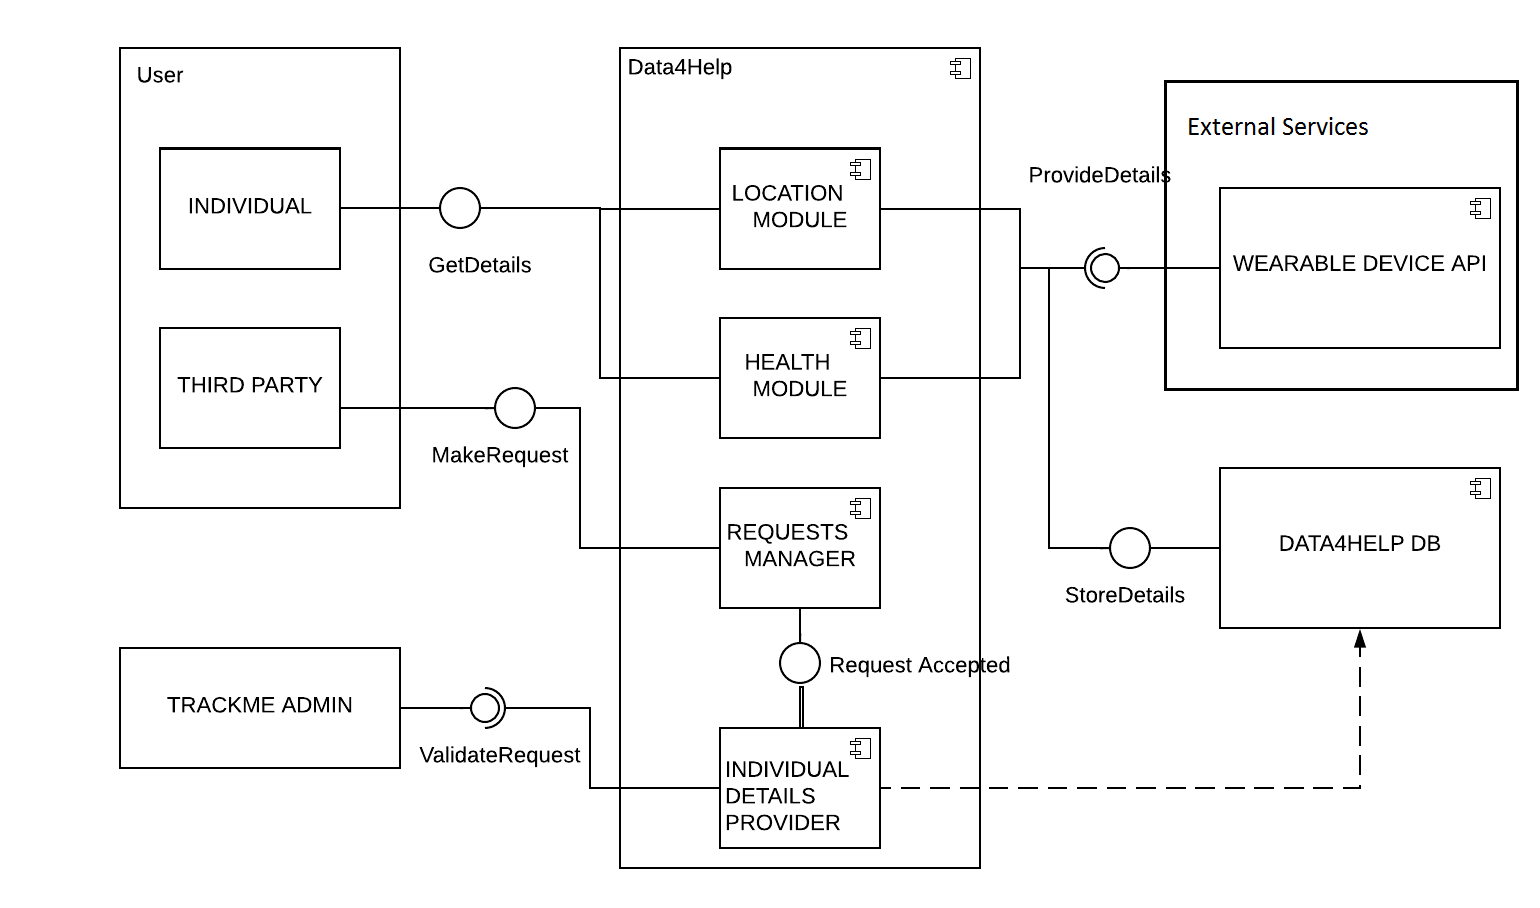
\includegraphics[width=\textwidth]{./DD_Diagrams/ComponentData4Help.png}
      	\caption{Component Diagram for Data4Help Service}
        \label{TrackMe_c1}
	\end{center}
\end{figure}

\begin{itemize}
\item\textbf{Location module:}  the location fetched from the Wearable Device API provided by an Individual is stored in the Data4Help DB.
\item\textbf{Health module:}  the health values fetched from the Wearable Device API provided by an Individual is stored in the Data4Help DB.
\item\textbf{Request Manager:}  provides an interface to the Third Party to make new request to get the details of a specific Individual or a group of Individual. It also provides an interface to a specific Individual to accept or reject the request.
\item\textbf{Individual Details Provider:} this uses the  help of the Data4Help DB to provide the details to the Third Party after the TrackMe Admin has validated the request.
\newline
\end{itemize}
\textbf{AUTOMATEDSOS SERVICE}
\begin{figure}[H]
	\begin{center}
		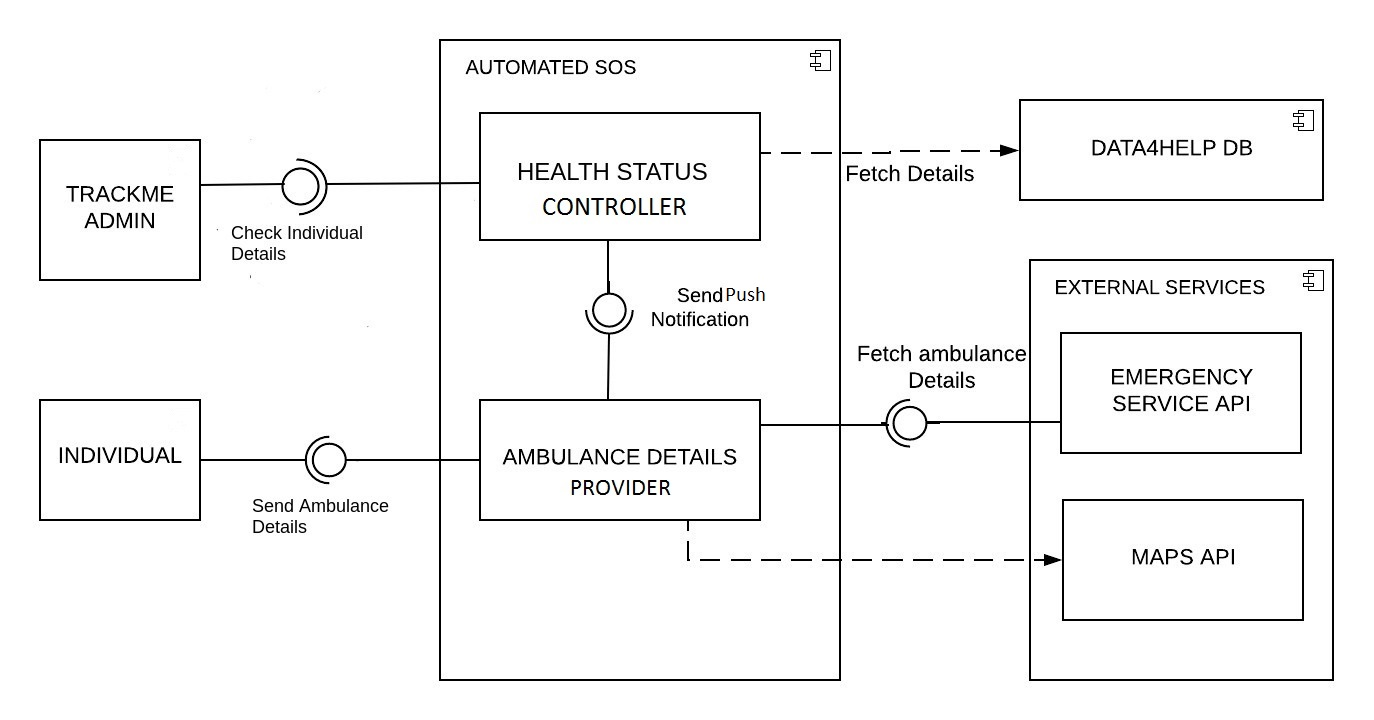
\includegraphics[width=\textwidth]{./DD_Diagrams/ComponentAutomatedSOS.jpg}
      	\caption{Component Diagram for AutomatedSOS Service}
        \label{TrackMe_c2}
	\end{center}
\end{figure}

\begin{itemize}
\item\textbf{Health Status Controller:}  uses the help of the Data4Help DB to get the details of an Individual. The TrackMe Admin provides an interface check Individual Details to the controller. The controller then, monitors the individual's vitals and when the vital is below the threshold value, it provides an interface named send notification.  
\item\textbf{Ambulance Details Provider:} gets the details of all the Ambulance associated to the major hospitals from the Emergency Service API. It uses the maps API to get the nearby ambulances and send notification to that ambulance driver application. It uses the functionality of Push Notification to send the notification. After a driver accept the request, the details of the driver is send to the Individual. 
\newline
\end{itemize}
\textbf{TRACK4RUN SERVICE}

\begin{figure}[H]
	\begin{center}
		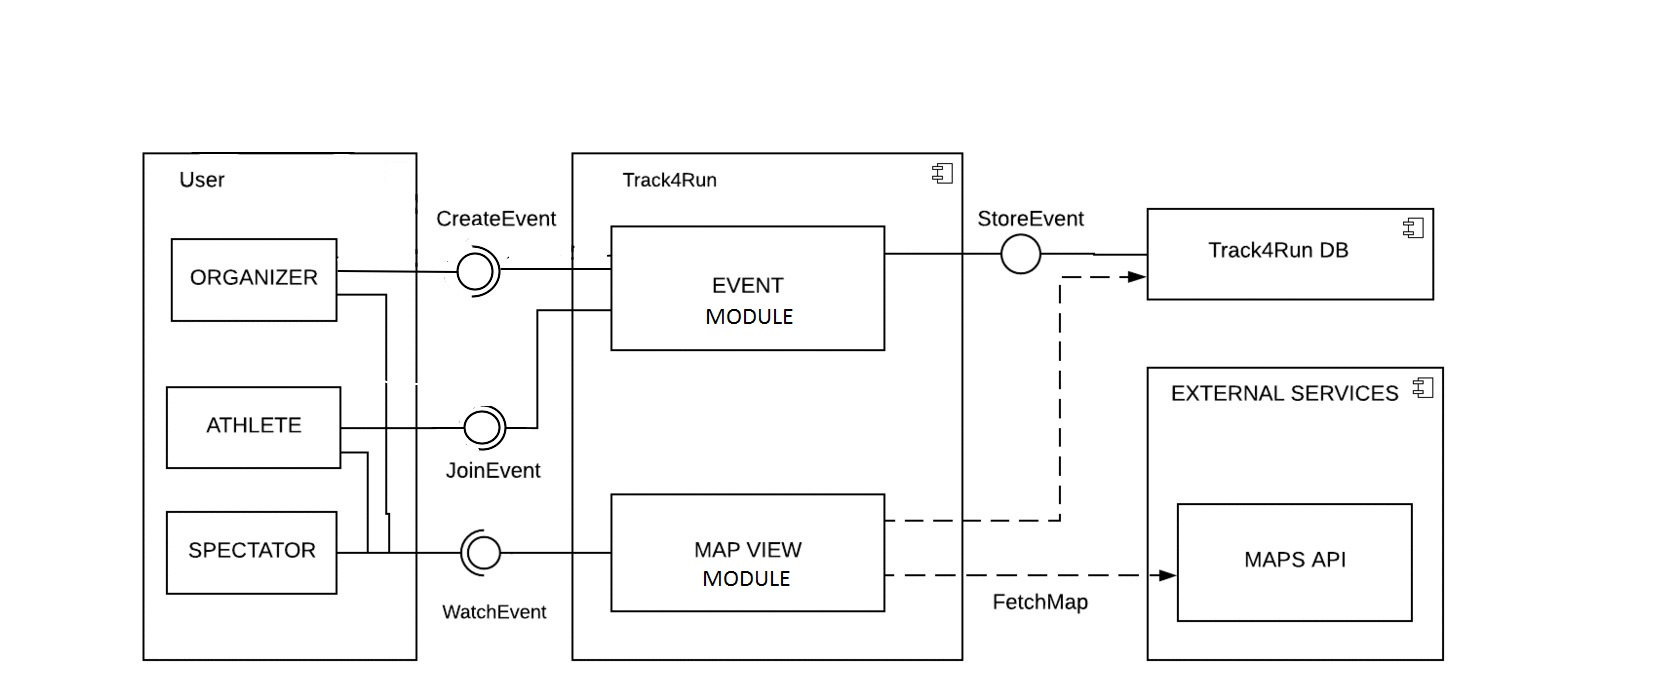
\includegraphics[width=\textwidth]{./DD_Diagrams/ComponentTrack4Run.jpg}
      	\caption{Component Diagram for Track4Run Service}
        \label{TrackMe_c3}
	\end{center}
\end{figure}

\begin{itemize}
\item\textbf{Event Module:} manages the details of the event and the athletes. It gets all the details of the event from the organizer which is entered after the organizer upgrades to the service. The event details is stored in the Track4Run DB. The athlete joins the event and is then associated with that specific event. 
\item\textbf{Map View Module:} It uses the Map API to provide an interface watch event to the organizer, athlete and the spectator. It checks the validity of the subscribed users. It uses the Track4Run DB to get the location of the athletes participating in an event, and then maps it to the interface.
\newline\newline\newline\newline\newline
\end{itemize}
\textbf{MAIN COMPONENT}

\begin{figure}[H]
	\begin{center}
		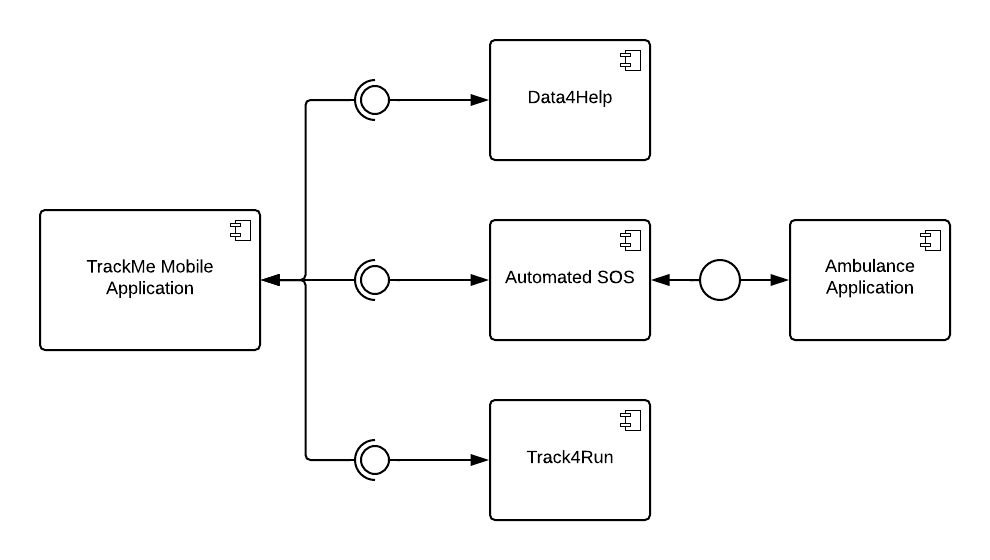
\includegraphics[width=\textwidth]{./DD_Diagrams/Component.png}
      \caption{Main Component Diagram}
        \label{TrackMe_c0}
	\end{center}
\end{figure}
The main component is divided into three subcomponents which are shown separately to avoid unreadability. All the three subcomponents are the services which is being provided by the TrackMe Application.\newline
The Ambulance Application is a separate application developed explicitly for the ambulance drivers where they receive individuals details through push notification. It is connected to Automated SOS service for exchange of information of ambulance and individual respectively.

\section{Deployment View}
\begin{figure}[H]
	\begin{center}
		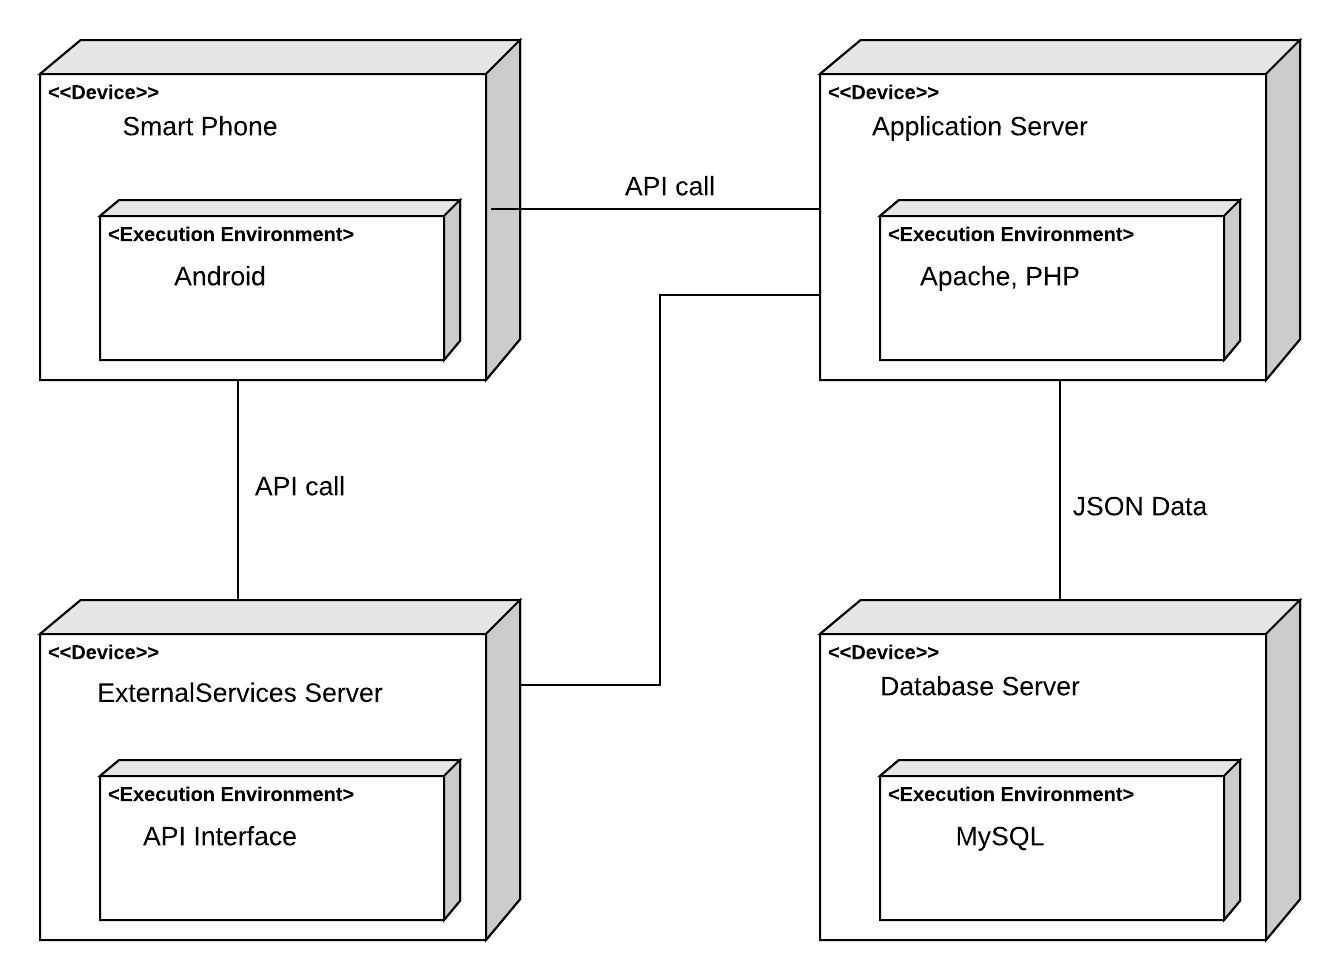
\includegraphics[width=\textwidth]{./DD_Diagrams/Deployment.png}
      \caption{Deployment Diagram}
        \label{TrackMe_depdia}
	\end{center}
\end{figure}
It shows architecture of the system as deployment (distribution) of software artifacts to deployment targets. Artifacts represent concrete elements in the physical world that are the result of a development process which are \textit{Android, Apache, PHP, API Interface} and \textit{MySQL}. Deployment target is usually represented by a node which is either hardware device or some software execution environment which are \textit{Smart Phone, Application Server, External Service Server} and \textit{Database Server}. The nodes are connected through communication paths to create networked systems of arbitrary complexity.\newline
The nodes an their respective artifacts are explained below:
\begin{itemize}
\item \textbf{Smart Phone:} The user uses smart phone to view the mobile application of the system. This is implemented in the execution environment Android which is artifact of this device.\newline
-\textit{Android:} The Android application can be built using any platform. It takes the information from external API's and the database server of the application to process and show information to the user using XML design techniques and Java Script codes.
\item \textbf{Application Server:} The Application Server is the host of the application and the database server. It is the central system of the entire application which manages the transfer and retrieval of data. The execution environment here is Apache and PHP.\newline
-\textit{Apache and PHP: } The Server does all the transaction on the database and manages the retrieval and transfer of data from and to database by using PHP code. We use PHP code to help convert the database into an API in JSON format which can be easily used by the application's front end to use the data.
\item \textbf{Database Server:} It stores all the data which is used by the application. The execution environment is MySQL.\newline
-\textit{MySQl:} MySQL database is used to store the details where the data can be easily stored from the form the user fills in the application. 
\item \textbf{ExternalServices Server:} It contains the information of all the external servers required by the application. The information from the server by using the API Interface.\newline
-\textit{API Interface:} The API provides the data in the JSON format which is fetched in the android platform by API call. 


\end{itemize}



\section{Runtime View}
The runtime view is explained with the help of sequence diagrams, which shows the interaction between the components during runtime in a time flow depicting the order of which function takes place after another. The function names are same as the interface in order to help to relate the component, their interaction and their behavior during runtime. The sequence diagram of the three major services of TrackMe are shown which comprises the entire functioning of TrackMe and integrates to make the complete application.\newline
Here are the three sequence diagrams which briefly summarizes the runtime of the application.
\begin{figure}[H]
	\begin{center}
		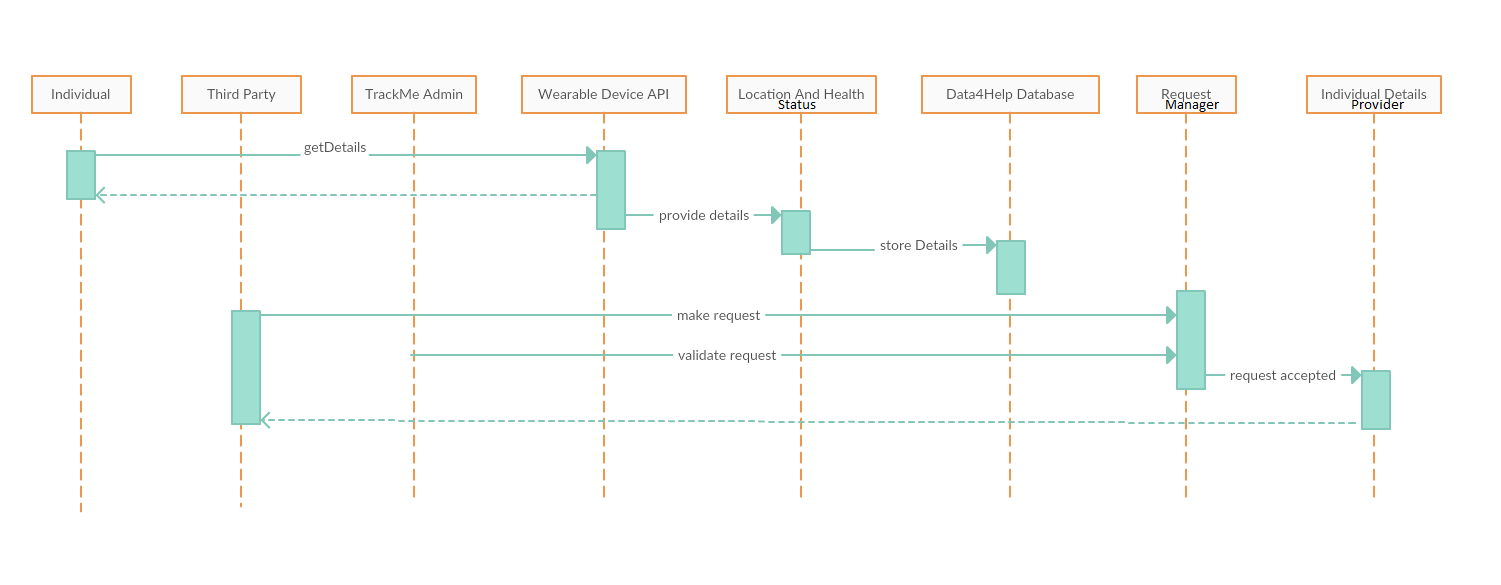
\includegraphics[width=\textwidth]{./DD_Diagrams/RuntimeData4Help.png}
      \caption{Sequence Diagram depicting runtime of Data4Help Service}
        \label{TrackMe_r1}
	\end{center}
\end{figure}
The location and health is taken from the user by the \textit{GetDetails Interface}  with the help of the API of the wearable device by \textit{ProvideDetails Interface}, which the individual selects from the list of compatible devices during registration. The details of the individual is then stored in the Data4Help database using \textit{StoreDetails Interface}.\newline
The thirdparty makes the request to access individual's data which is done by \textit{MakeRequest Interface}.\newline
The TrackMe Admin then validates the third party request and sends it to user to accept/reject or accepts/rejects himself according to the type of requests by \textit{ValidateRequest Interface}.\newline
If the request is accepted the user gets the access of the individual's details which uses the Data4Help Database in order to extract individual's details.
\begin{figure}[H]
	\begin{center}
		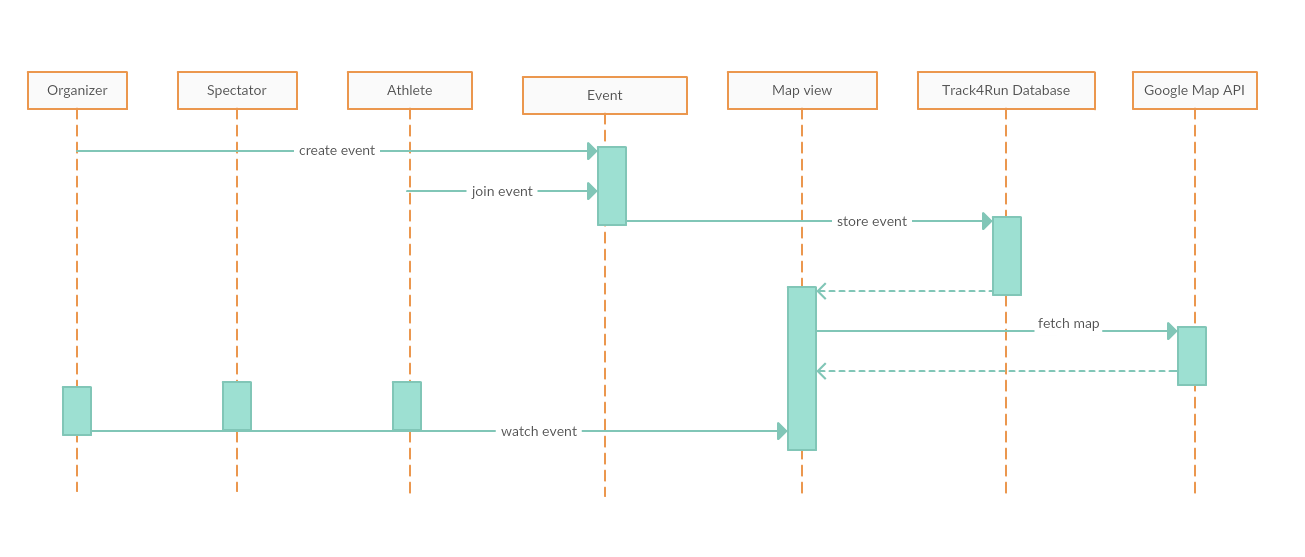
\includegraphics[width=\textwidth]{./DD_Diagrams/RuntimeAutomatedSOS.png}
      \caption{Sequence Diagram depicting runtime of AutomatedSOS Service}
        \label{TrackMe_r2}
	\end{center}
\end{figure}
Trackme checks the age of the user in order to know whether they are eligible for this service and checks the vitals to know about the emergency condition using  using \textit{CheckIndividualDetails Interface} which is fetched from the Data4Help Database and updated as Health Status component which contains the emergency vitals of individuals.\newline 
If the emergency situation is acknowledged the admin sends notification using \textit{SendPushNotification Interface} which includes the health status and location.\newline
The Individual receives the Ambulance Details by \textit{SendAmbulanceDetails Interface} and can track the ambulance whose information is fetched from the emergency Service API using \textit{FetchAmbulanceDetails Interface} and uses Maps API to show the map.
\begin{figure}[H]
	\begin{center}
		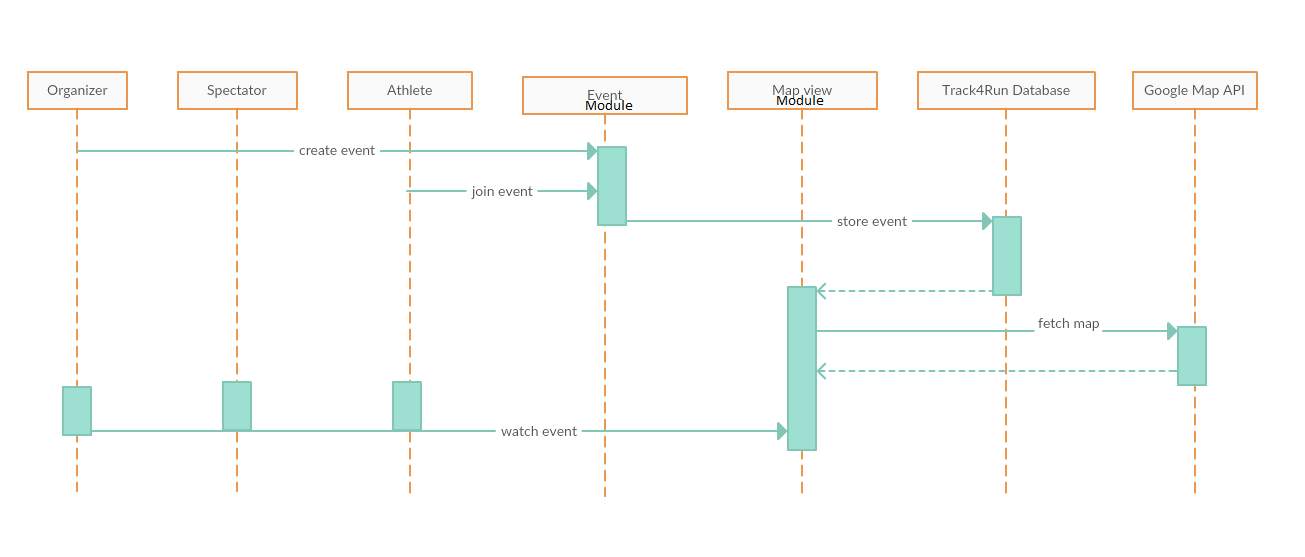
\includegraphics[width=\textwidth]{./DD_Diagrams/RuntimeTrack4Run.png}
      \caption{Sequence Diagram depicting runtime of Track4Run Service}
        \label{TrackMe_r3}
	\end{center}
\end{figure}
The organizer creates an event which the athlete joins using \textit{CreateEvent Interface} and \textit{JoinEvent Interface} respectively. The details of the event is store din the Track4Run Daatabase using \textit{StoreEvent Interface} which is used by Map view to show the details on map. The organizer, athlete and Spectator can watch the race in a map using \textit{WatchEvent Interface} which uses Map API to fetch the map.

\section{Component Interfaces}
In the following diagrams, the component interfaces are presented and the dependencies between the parts of the application server are shown. Each Interfaces which is already explained in the runtime view are detailed here with all the functions and methods they include. Like the component diagram, has three parts to implement three services in the same manner this has three separate diagram to explain all the interfaces and there interactions.
\begin{figure}[H]
	\begin{center}
		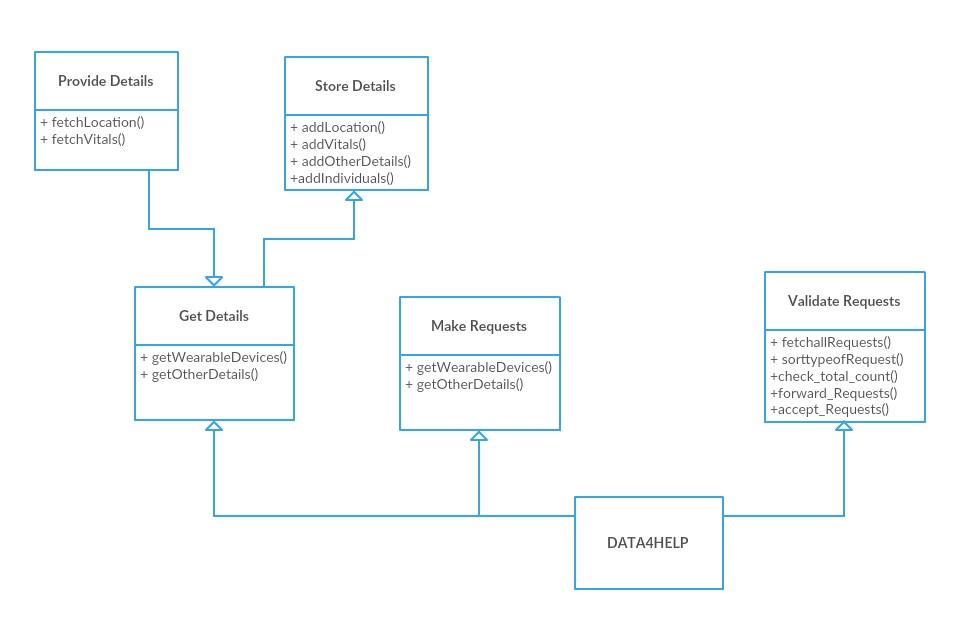
\includegraphics[width=\textwidth]{./DD_Diagrams/InterfaceData4Help.jpg}
      \caption{Component Interface Diagram for Data4Help}
        \label{TrackMe_int1}
	\end{center}
\end{figure}
\begin{figure}[H]
	\begin{center}
		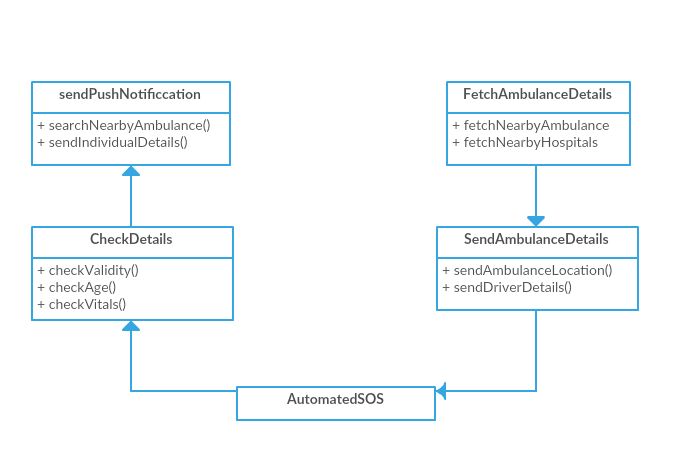
\includegraphics[width=\textwidth]{./DD_Diagrams/InterfaceAutomatedSOS.png}
      \caption{Component Interface Diagram for AutomatedSOS}
        \label{TrackMe_int2}
	\end{center}
\end{figure}
\begin{figure}[H]
	\begin{center}
		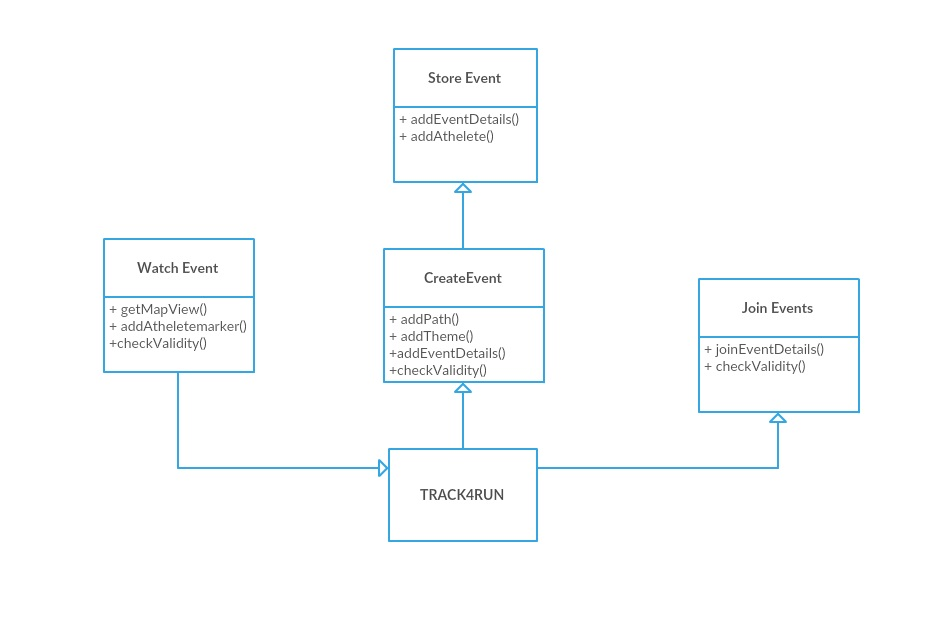
\includegraphics[width=\textwidth]{./DD_Diagrams/InterfaceTrack4Run.jpg}
      \caption{Component Interface Diagram for Track4Run}
        \label{TrackMe_int3}
	\end{center}
\end{figure}

\section{Selected architectural styles and patterns}
\subsection{Overview}

\qquad The system essentially uses a variety of the multi-layered architecture i,e is the three-tired architecture for our TrackMe application. The application includes a presentation layer, business layer and data layer. The presentation layer, which is the top most layer represents the  display of information related to the services given by the application like checking health status, requesting data, watching a live race etc. The presentation layer directly interacts with the client getting information from the client, with the help of GUI. The business layer also known as the application layer in general, fetches the details form the presentation layer and does detailed processing. For instance it ensures the connection with the corresponding external services required and processing for the data from the services like Google maps, wearable devices etc. The data access layers basically provides an API to the application tier that exposes methods of managing the stored data without exposing or creating dependencies on the data storage mechanisms.

\par We use a three tier application so that we would be able to update the technology stack of one tier without affecting the other one, and provides an easy of managing the different layers.

\subsection{Design Patterns and Architectural Choices}
\begin{enumerate}
\item Push Notification
\par We have used the push notifications, which include the location and details of the individuals in need of emergency care are send to the ambulance drivers via the ambulance application. We basically use the application to make sure of the time constraints that the notification should reach within 5 seconds. The choice is made because of the difficulty in coming up with an asynchronous protocol for message exchanging.
\item Robustness 
\par The principal usage of the system is done through mobile applications which are running on mobile terminals. As we can imagine, in that domain the robustness of the system is an important aspect to keep in
mind. The mobile devices are often subject to loss of connectivity and for that reason the communication between the server and a client could be not available in various time points
\end{enumerate}


\subsection{Other Design Decisions}
\begin{enumerate}
\item Storage of Passwords
\par The passwords are not stored in plain-text but they are hashed and salted with cryptographic hash functions. This provides a last line of defense in case of data theft.
\item Programming Languages
\par For the implementation of TrackMe application we choose Java as a programming language. This choice is based on the following considerations:
	\begin{enumerate}
	\item Java is a widespread programming language, so we are sure that there will be availability of skilled programmers in this technology.
    \item The choice of the platform is left to the developer. He/she has wide range of Java platforms to choose from.
	\end{enumerate}
\item Ambulance Mobile Application
\par The ambulance mobile application has been developed basically for the ambulance drivers to recieve the above mentioned push notification within a time interval of 5 seconds.
\item External Services
\par The system uses external services, Google Maps to offload all geo-localization, position tracking and map visualization process. The reasons of the choice are the following:
	\begin{enumerate}
	\item Manually developing maps for city of Milan is not a viable option due to tremendous amount of coding and data collection time required.
    \item Google Maps is a well-established, tested and reliable software component used by millions of people used around the world.
    \item Google Maps can be used both on the server side and the client side. 
    \item Users feel comfortable using a software which they daily use it.
    \item Google Maps offers API, enabling programmatic access to features.
	\end{enumerate}
    
\par The system also uses external services like wearable device API, which helps us to fetch the health vitals of the patients and the emergency service API to extract all the details of the nearby hospitals. Wearable device are the best choice to get the health vitals of a patient as it is easy to have it on hand always and can be easily connected to the application. Most of the users will be having a prior experience to use a wearable device.
\end{enumerate}



%%%%%% USER INTERFACE DESIGN %%%%%%%%
\chapter{User Interface Design}
\label{ch:user_interface_design}
The following User-Interface flow diagram enable us to model the high-level relationships between major user interface elements that are described in our RASD documents. It is used to organize the activities of TrackME application into groups and have an overview of the interfaces and interactions. \newline

\begin{itemize}
\item The user interface for an individual allows the individual to view the vitals, view the third party details, and accept/reject the request.
\begin{figure}[H]
	\begin{center}
		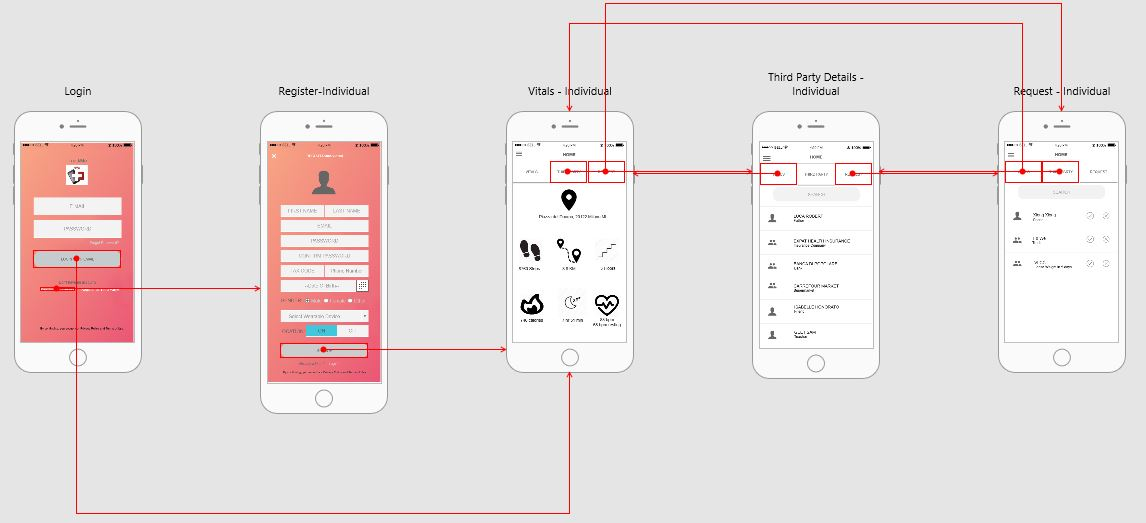
\includegraphics[width=\textwidth]{./DD_Diagrams/UI_Individual.JPG}
        \caption{User Interface - Individual}
        \label{ui_individual}
	\end{center}
\end{figure}
\end{itemize}

\begin{itemize}
\item The user interface for a Third Party allows the third party to view the details of the individual viewed in a pop-up box, allows to make new request, and view the status of the request already made.
\begin{figure}[H]
	\begin{center}
		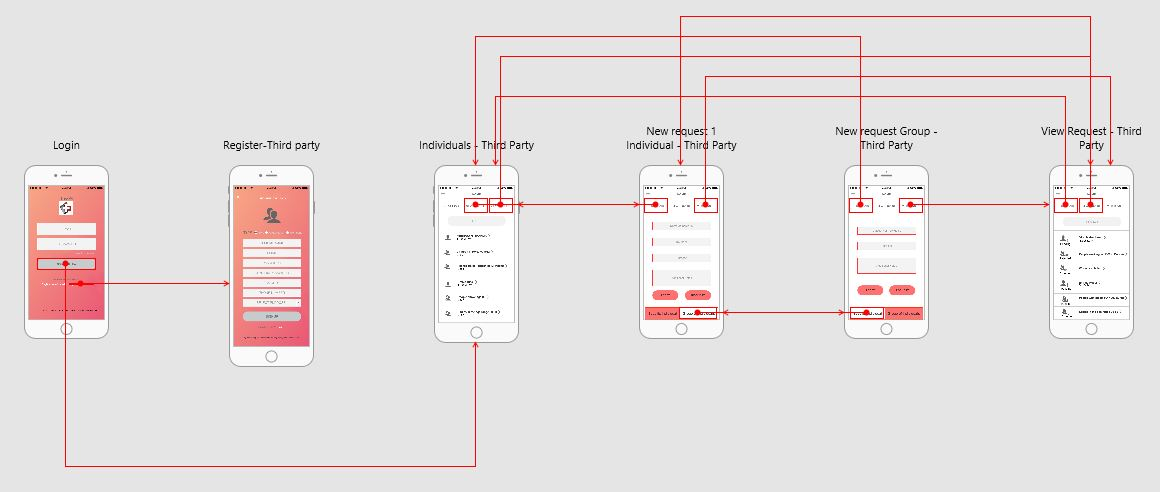
\includegraphics[width=\textwidth]{./DD_Diagrams/UI_ThirdParty.JPG}
        \label{ui_thirdparty}
        \caption{User Interface - Third Party}
	\end{center}
\end{figure}
\end{itemize}

\begin{itemize}
\item The Menu Interface allows an user to view their own profile, upgrade to a new service, and then allow to view the new service.
\begin{figure}[H]
	\begin{center}
		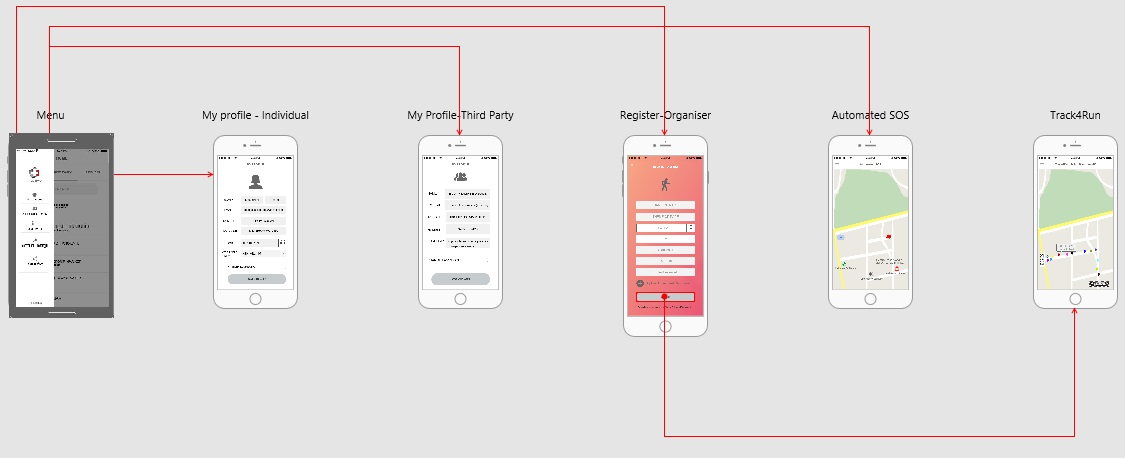
\includegraphics[width=\textwidth]{./DD_Diagrams/UI_Menu.JPG}
        \caption{User Interface - Menu}
        \label{ui_menu}
	\end{center}
\end{figure}
\end{itemize}




%%%%%% REQUIREMENTS AND TRACE ABILITY %%%%%%%%
\chapter{Requirements Traceability}
\label{ch:requirement_traceability}

The main objective of determining the design described in this document was to fulfill the requirements and goals mentioned in the Requirement Analysis and Specific Documents.\newline
The following list outline the mapping between the requirement and goals with the design elements mentioned in the DD.\newline

\begin{itemize}

\item\textbf{[G1]} Providing a list of the wearable devices that an individual can choose from. ([R1]-[R2])
\begin{itemize}
\item Data4Help
\begin{itemize}
\item Location Module
\item Health Module
\item Wearable Device API
\item Data4Help DB
\end{itemize}
\end{itemize}

\item\textbf{[G2]} Expedite the request made by the 3rd party to an individual to access their details. ([R3]-[R4])
\begin{itemize}
\item Data4Help
\begin{itemize}
\item Request Manager
\item Data4Help DB
\end{itemize}
\end{itemize}

\item\textbf{[G4]} Validating the request made by the 3rd party to provide the details of a group of individuals.([R6]-[R8])
\begin{itemize}
\item Data4Help
\begin{itemize}
\item Request Manager
\item Individual Details Provider
\item Data4Help DB
\end{itemize}
\end{itemize}

\item\textbf{[G5]} Quick access of the data to the 3rd party once the request is approved.([R9]-[R10])
\begin{itemize}
\item Data4Help
\begin{itemize}
\item Request Manager
\item Individual Details Provider
\item Data4Help DB
\end{itemize}
\end{itemize}

\item\textbf{[G6]} Immediate update of the data once an individual updates their own details.([R11]-[R12])
\begin{itemize}
\item Data4Help
\begin{itemize}
\item Location Module
\item Health Module
\item Wearable Device API
\item Data4Help DB
\end{itemize}
\end{itemize}

\item\textbf{[G8]} Monitoring the health status of the subscribed individual to the Automated SOS service.([R14]-[R16])
\begin{itemize}
\item AutomatedSOS
\begin{itemize}
\item Health Status Controller
\item Ambulance Details Provider
\item Data4Help DB
\item Emergency Service API
\item Maps API
\end{itemize}
\end{itemize}

\item\textbf{[G9]]}  Develops an interface to organize a race for the subscribed 3rd party to the Track4Run service.([R17]-[R19])
\begin{itemize}
\item Track4Run
\begin{itemize}
\item Event Module
\item Track4Run DB
\end{itemize}
\end{itemize}

\item\textbf{[G10]} Give access to the details of the race once an individual participate in it.([R20]-[R21])
\begin{itemize}
\item Track4Run
\begin{itemize}
\item Event Module
\item Track4Run DB
\end{itemize}
\end{itemize}

\item\textbf{[G11]} Live visualization of the race .([R22]-[R23])
\begin{itemize}
\item Track4Run
\begin{itemize}
\item MapView Module
\item Track4Run DB
\item Maps API
\end{itemize}
\end{itemize}

\end{itemize}

%%%%%% Implementation Integration and TestPlan %%%%%%%%
\chapter{Implementation, Integration and Test Plan}
\label{ch:implementaion_intergrationandtestplan}

\section{Implementation}
The implementation of the TrackMe system will be done service by service followed with the integration of all the services. The order in which it is be carried out depends on a number of factors like the complexity of the modules and services, the dependence of other modules on the component being implemented and to the system as a whole, and it should also take into account the possibility of discovering flaws with the proposed design. The later should be dealt in a way that, if such an unfortunate event does happen,the flaws should be found and corrected as soon as possible, to limit the cost of the change of design. 
In this sense, the components of the TrackMe, could be grouped in the following way, with the order specifying the order of implementation: \newline
1. Data4Help Service\newline 2. Automated SOS Service and Ambulance Application\newline 3. Track4Run Service\newline 4. TrackMe (Connecting the above three services)\newline

The first service to be built is Data4Help Service as the further services exploits the features of Data4Help Service. Data4Help is a base service which all the individuals and third party will have by default when they register in the application. Hence, it has to be built first as a separate service. This service does the main function of taking data from user and storing it in database and hence does not require any payment interface with might be required by other services, hence it is implemented separately.\newline 

After the first service AutomatedSOS and TrackMe Ambulance Application is implemented which is a service used by only Individuals. This is a service for the elderly individuals whose vitals are monitored and a nearby ambulance is sent whenever emergency situations are encountered. This service exploits the features of the above service and hence it is implemented after that. The details of the individuals with vitals below threshold is sent to the Ambulance Driver. The ambulance drivers have explicit applications in order to ensure fast delivery of individual's data through push notification.Hence the application must be implemented together with this service layer as there is an exchange of information from application to this service layer and vice versa.\newline

The next service implemented is Track4Run service which is basically an event which is organized by Organizers who are basically third party and individuals can perform as athlete. This service is not related to the second service by any means and hence both the services can be implemented parallely and separately and this can be implemented even before AutomatedSOS. The order of these two service wont matter but it must be implemented after Data4Help Service as it exploits the feature of that service as well.\newline

After implementing all the three services of the application, we can merge them and implement the entire working of the application connecting all the three services and how the user upgrades from Data4Help to other services and uses them. Hence this layer is implemented at the end after implementing all the services separately.

\section{Integration}
\textbf{1. Integration of Data4Help} 
\begin{itemize}
\item Integration of the components of Data4Help of the application server.\newline
-- Request Manager, Individual Details Provider
\item Integration of components of Data4Help with the DBMS. \newline
-- Location Module, Data4Help DB\newline
-- Health Module, Data4Help DB\newline
-- Individuals Details Provider, Data4Help DB
\item Integration of components of Data4Help with the (other) external services. \newline
-- Location Module, Wearable Device API\newline
-- Health Module, Wearable Device API\newline
\end{itemize}
\textbf{2. Integration of Automated SOS}
\begin{itemize}
\item Integration of the components of Automated SOS of the application server.\newline
-- Health Status Controller, Ambulance Details Provider
\item Integration of components of Automated SOS with the DBMS. \newline 
-- Health Status Controller, Data4Help DB
\item Integration of components of Automated SOS with the (other) external services. \newline
-- Ambulance Details Provider, Emergency Services API\newline
-- Ambulance Details Provider, Maps API\newline
\end{itemize}
\textbf{3. Integration of Track4Run}
\begin{itemize}
\item Integration of components of Track4Run with the DBMS. \newline 
-- Event Module, Track4Run DB
\item Integration of components of Track4Run with the (other) external services. \newline
-- Map View Module, Track4Run DB
-- Map View Module, Maps API
\end{itemize}
\textbf{4. Integration of TrackMe}
\begin{itemize}
\item Integration of the components of TrackMe with Data4Help.
\item Integration of components of TrackMe with AutomatedSOS. 
\item Integration of components of TrackMe with Track4Run. 
\item Integration of AutomatedSOS with TrackMe Ambulance Application.
\end{itemize}

\section{Integration Test Plan}
\begin{figure}[H]
	\begin{center}
		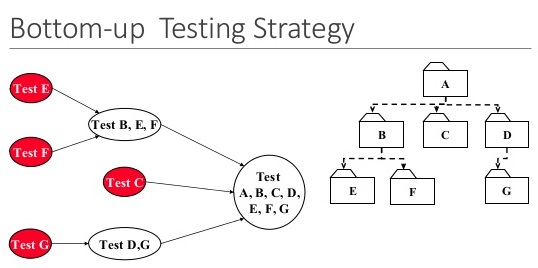
\includegraphics[width=\textwidth]{./DD_Diagrams/testplan2.jpg}
      \caption{Bottom up- strategy for testing integration plan}
        \label{TrackMe_tp2}
	\end{center}
\end{figure}
A bottom-up approach is the piecing together of systems to give rise to more complex systems, thus making the original systems sub-systems of the emergent system. Bottom-up processing is a type of information processing based on incoming data from the environment to form a perception. From a cognitive psychology perspective, information enters the eyes in one direction (sensory input, or the "bottom"), and is then turned into an image by the brain that can be interpreted and recognized as a perception (output that is "built up" from processing to final cognition). In a bottom-up approach the individual base elements of the system are first specified in great detail. These elements are then linked together to form larger subsystems, which then in turn are linked, sometimes in many levels, until a complete top-level system is formed. This strategy often resembles a "seed" model, by which the beginnings are small but eventually grow in complexity and completeness. However, "organic strategies" may result in a tangle of elements and subsystems, developed in isolation and subject to local optimization as opposed to meeting a global purpose.\newline
Considering the implementation plan and the overall architecture of the TrackMe application, the chosen strategy for the integration testing is the \textit{bottom-up strategy}. This allows us to start the integration and it’s testing while not waiting for the completion of the development and the unit testing of each component in the system. Considering the integration of two components, we would assume that, in best case, they have been implemented fully and that their respectful unit tests pass. However, the integration can, in some cases, start, if necessary, before the implementation has been completed. This can be allowed if the part of the component needed for that specific integration has been completed and tested. \newline

Since the opted solution is to start from the bottom-up, that means that the among the first integrations performed will have the already built external components in them. Since the application rests on these services and the communication with them, this order of integration and testing will enable the earlier detection of errors in these critical parts. 
\begin{figure}[H]
	\begin{center}
		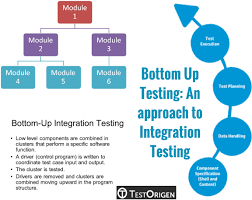
\includegraphics[width=\textwidth]{./DD_Diagrams/testplan.png}
      \caption{Working of bottom up- strategy for testing integration plan}
        \label{TrackMe_tp}
	\end{center}
\end{figure}

%%%%%% EFFORT SPENT%%%%%%%%
=======
The document represents the Requirement Analysis and Specification Document for the application named TrackMe. TrackMe is an web/android application that provides a certain services like vital monitoring, emergency services for elderly people and real time visualization of race or marathons. 

This document focuses to completely describe the TrackMe system in terms of functional and non-functional requirements, analyze the real needs of the customer in order to model the system. We also focus on the constraints and the limitations of the software to indicate the typical use cases. 

Further, this document will provide formal specification of some features of the applications, by means of the Alloy language~\cite{alloy-site}.

The document is addressed to both the customers which specifies the requirements as mentioned by the customers and the developers who have to implement the requirements.
>>>>>>> 113baf26200f5cdcd76ad522dfc4e5917a715c40

\section{Scope}
Track4Me is a company which provides three software based services. The services are limited to the citizens of Milan. The given problem is to design and develop a software service called  “Data4Help”,  which acts as an intermediary between the individuals and the other companies. It targets two set of users, individuals and third party. The location and health of the user is extracted from a wearable device. The data from the wearable device is extracted with the help of the API of the wearable device. The software tracks the location and health status of individuals or group of individuals and send the information to the third party on their request to monitor the health of individuals by validating the type of requests. The validation of the requests for the information of specific individuals is done by the individual’s self acceptance or rejection. The requests for the information of group of individuals is decided by Track4Me and generalized by allowing the access to the third party, if the number of individuals whose information is to be accessed is greater than 1000.

It builds a new service called “AutomatedSOS” over the top of “Data4Help” after monitoring the demand of requests from third parties for giving non-intrusive SOS service to elderly people, which sends the ambulance to individual’s location when the health parameters are below the thresholds. The nearest ambulance is tracked and sent to ensure individual’s quick and efficient recovery. A separate mobile application of Track4Me is to be exclusively developed for the ambulance drivers who are informed by push notifications in the mobile application along with the location and other details of the patient in less than 5 seconds to ensure spontaneity in reaction to emergencies. All the hospitals in Milan are informed to ensure all the ambulance drivers installs TrackMe application.

A new service called “Track4Run” is built as a source of revenue which allows organizer to organize an event, athletes to participate in the event and spectators to see the athletes position live in a Map. It exploits the service of “Data4Help” which tracks the location of the athletes to be visible to everyone and helps the organizer to monitor the health status of athletes as well. The organizer will be registered as an existing or new third-party. The athletes will be registered as existing or new individual and the spectators can be registered as new/existing individual/third party.

The users can either register as an individual or as an organization/ company (third party). Data4Help is a base service which all the individuals and third party will have by default even if the user registers for a different service other than “Data4Help”. The third party can register for two services: “Data4Help” and “Track4Run”. It uses “Data4Help for receiving information about targeted individuals and “Track4Run to organize events for a particular cause/occasion. The third party is a source of revenue for both cases, as Track4Me provides information about individuals and thereby,  provides customers to their organization which brings them profit. Individuals can register for any of the three services. The first service is a free service  with a motive to help them to receive specific input from respective third party for their health issues or other factors. The individual can also upgrade to other services if they are an existing a member using one service by making payment. Payment can be made using PayPal or a credit card. Track4Me guarantees the security of the individuals data and only associates with trusted third party companies. Ultimately, it helps both individuals and third party to manage and monitor their personal data and aims at being a robust and efficient software.


\section{Goals}
\begin{itemize}
\item \textbf{[G1]} Providing a list of the wearable devices that an individual can choose from.
\item \textbf{[G2]} Expedite the request made by the 3rd party to an individual to access their details.
\item \textbf{[G3]} Provides an interface for an individual to analyze the request made by the 3rd party.
\item \textbf{[G4]} Validating the request made by the 3rd party to provide the details of a group of individuals.
\item \textbf{[G5]} Quick access of the data to the 3rd party once the request is approved.
\item \textbf{[G6]} Immediate update of the data once an individual updates their own details.
\item \textbf{[G7]} Provides an up-gradation to the new services, Automated SOS or Track4Run.
\item \textbf{[G8]} Monitoring the health status of the subscribed individual to the Automated SOS service.
\begin{itemize}
\item \textbf{[G8.1]} Alerts the nearby ambulance, when the health status of the individual is low, within 5 seconds.
\end{itemize}
\item \textbf{[G9]} Develops an interface to organize a race for the subscribed 3rd party to the Track4Run service.
\item \textbf{[G10]} Give access to the details of the race once an individual participate in it.
\item \textbf{[G11]} Live visualization of race.
\end{itemize}




\section{Definitions, Acronyms, and Abbreviations}
\subsection{Definitions}
\begin{enumerate}
\item Services: Functionalities offered by the application
\item Validation: Verifying if requests provided by the 3rd party are genuine or not. If it is genuine it is accepted else rejected.
\item Upgrade: Enhancing the functionalities. 
\item Update: Adding new information or changing the previous one.
\item Threshold: A limit. Threshold on age has been kept for Automated SOS service.
\item Push Notification: The message that pops up on the Mobile. 
\end{enumerate}

\subsection{Acronyms}
\begin{enumerate}
\item RASD: Requirement Analysis and Specification Document
\item API: Application Program Interface
\item GPS: Global Positioning System
\item SOS: Save our Souls
\end{enumerate}

\subsection{Abbreviations}
\begin{enumerate}
\item Gn: n-Goals
\item An: n-Assumptions
\item Dn: n-Dependencies
\item Cn: n-Constraints
\item Rn: n-Functional Requirement s
\end{enumerate}


\section{References}
\begin{itemize}
\item Specification Document: "Mandatory Project Assignment AY 2018-2019.pdf"
\item Alloy model example: "http://alloytools.org/tutorials/online/"
\item Requirement Engineering Slides I, II
\item Alloy Slides 
\end{itemize}

\section{Document Structure}
\qquad The RASD is composed of 6 parts including references
\begin{enumerate}
\item Chapter 1 is an introduction to the problem which identifies the scope and goals of the application to be developed. Apart from this different definitions, acronyms and abbreviations used in the document are also noted down here.
\item Chapter 2 comprises of the overall description of the application which includes product functionalities, the users involved and the assumptions, dependencies and constraints.
\item Chapter 3 takes into the specific requirements like the interfaces used, functional requirements and the different unified modeling language diagrams and the non-functional requirements.
\item Chapter 4 contains the Alloy code and metamodel we have created.
\item Chapter 5 contains the effort spend by each of the Team Members.
\item Chapter 6 of the document has all the references.
\end{enumerate}

%%%%%% OVERALL DESCRIPTION %%%%%%%%
\chapter{Overall description}
\label{ch:overall-desc}

\section{Product perspective}
\subsection{Class Diagram}
\begin{figure}[H]
	\begin{center}	
		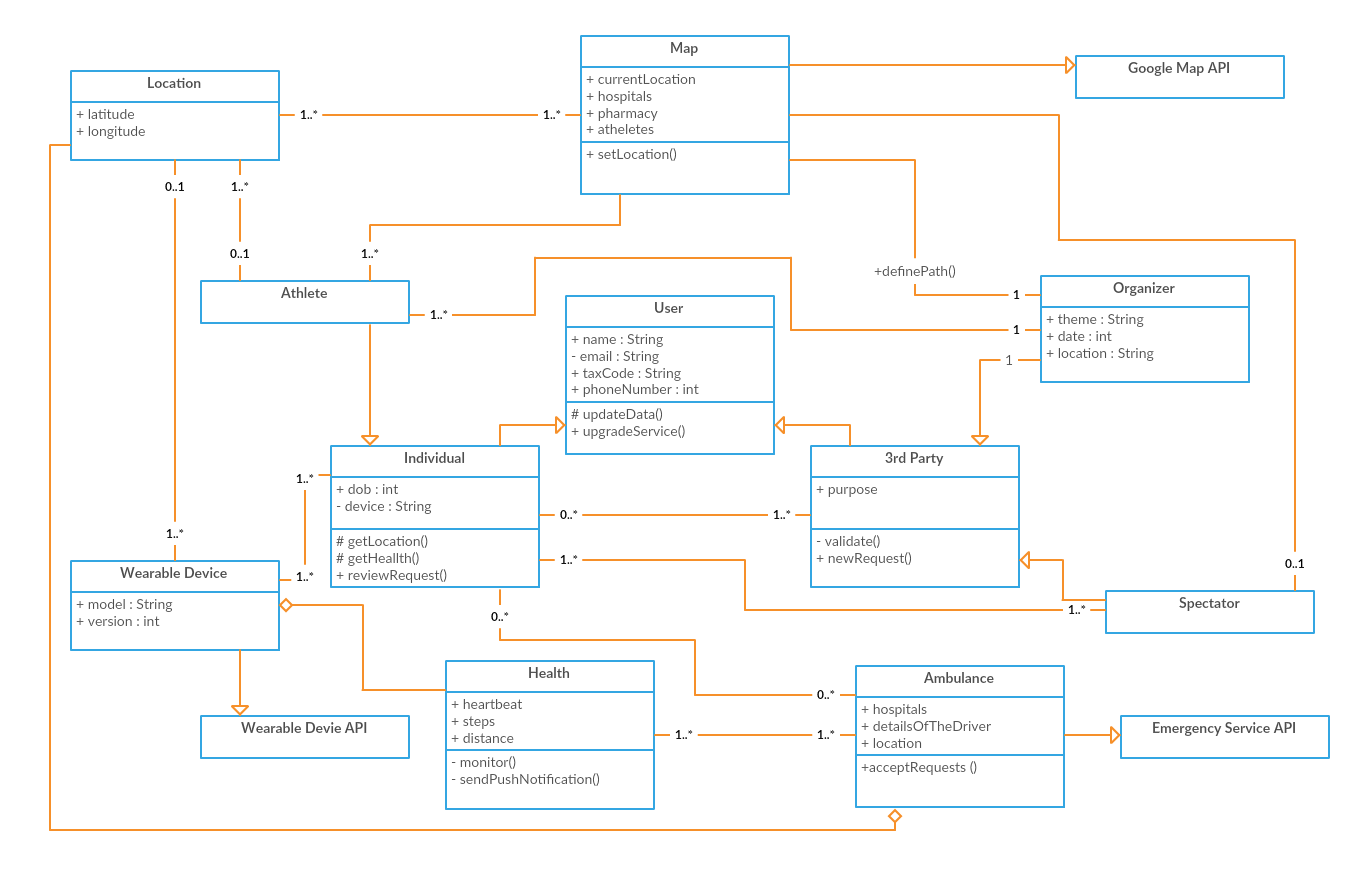
\includegraphics[width=\textwidth]{./RASD_Diagrams/ClassDiagram.png}
      	\caption{Class Diagram for TrackMe}
        \label{TrackMe_classdiagram}
	\end{center}
\end{figure}

%---------------STATE DIAGRAM----------------------%
\subsection{State Charts}
\begin{figure}[H]
	\begin{center}
		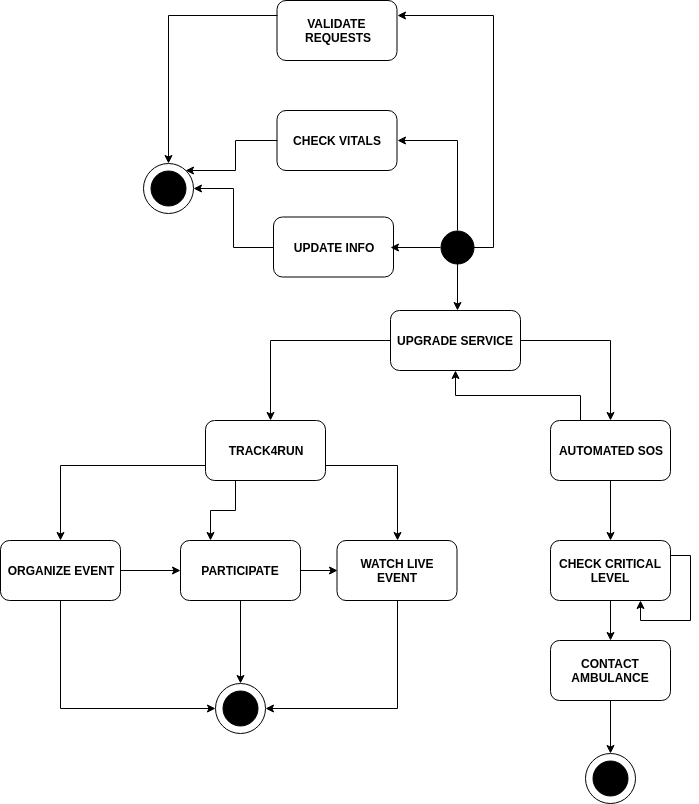
\includegraphics[width=\textwidth]{./RASD_Diagrams/StateDiagram.png}
      	\caption{State Diagram for TrackMe}
        \label{TrackMe_statediagram}
	\end{center}
\end{figure}

\section{Product functions}
\subsection{Vital Status}
\qquad TrackMe uses it service named Data4Help to share the health status of individuals to be monitored, to the third party on their requests. The health status of the individual will be extracted from a wearable device through the API of the wearable device about which the individual will mention while registering by selecting their device among the list of compatible wearable devices of TrackMe. The health parameters which are extracted includes heart beat rate, no. of steps, body temperature, detection of seizures, tremors etc. This is an important and crucial function of the software because it deals with individuals health and safety. Track4Me launches a new service called “AutomatedSOS” where TrackMe itself monitors the individual's health status and do the needful.

\subsection{Location Tracking}
\qquad Data4Help helps TrackMe to use monitor the location of the individual which can be later shared with the third party after validation. This service of location tracking can be helpful in case of emergencies which we come across in automated SOS. We basically use the Global Positioning System or the GPS to track the location of the individual. There are chances that we can lose the GPS connection in certain cases like may be inside our home due to poor connection to satellite. In such cases we can fetch the location from the nearest wi-fi to which our device get connected. In case of an emergency TrackMe system shall locate a minimum of 3 available ambulances that are closest to the emergency location by displaying a map and marking location of the emergency and ambulance nearby, which is would be taking less than a minute to fetch. We then share the data to the nearest ambulance within 5 seconds.We also use location tracking for athletes for a real time visualization of the positions of the athletes for a particular race which is explained further below.

\subsection{Third Party Validation}
\qquad In order to maintain the privacy of an individual customer, the 3rd party is validated by the system. The 3rd party has to provide a valid proof and request the data of an individual customer. The customer, in turn, gets all the details of the 3rd party that has requested their data. Customer decides whether to accept or refuse the request of the 3rd party. TrackMe handles the request made by the 3rd party, when the data requested is of a group of customers. The request is only approved when data requested is of more than 1000 customers.

\subsection{Organizing a Race}
\qquad TrackMe provides an interface for the subscribed 3rd party to organize a race.  An organizer needs to set realistic goals and mention a purpose of the race.  Then, an organizer has to select the location, date and time. The organizer needs to upload the Government Permission to organize a race. As an individual join the race organized by the organizer, the details of the individual is instantly available to the organizer. List View is provided of all the participants for the organizer.

\subsection{Expeditious Data Convey}
\qquad Track4Me monitors the health status themselves when the individual uses the service “AutomatedSOS” rather than sending the data to the third party to be monitored. When the health parameters go below the threshold, Track4Me tracks the location of the nearby ambulance to the patient. The nearby ambulance is tracked with the help of external emergency services API. The nearby ambulance drivers then receive a request through push notification and the one who accepts the request first goes to the location of the patient. A separate mobile application of Track4Me is to be exclusively developed for the ambulance drivers to send the location and other details of the patient in less than 5 seconds to ensure spontaneity in reaction to emergencies. All the hospitals in Milan are informed to ensure all the ambulance drivers installs TrackMe application.

\subsection{Real Time Visualization of Race}
\qquad This service is basically used by the spectators who wish to watch a race or marathon live, which comes as a part of the Track4Run. Once an athlete registers with the Track4Run service. His/Her location is tracked live with the help of the device using GPS. Track4Run fetches the track details way before and set it as the Track for a particular race or marathon and shows an enlarged view of the track while displaying the live positions of the participants.

\section{User characteristics}
\subsection{Admin}
Admin is the TrackMe application and the team handling the operations of the application. All the functions handled and done by TrackMe is denoted here to be done by the admin.
\subsection{Individual}
A person using TrackMe for monitoring his/her vitals using the Data4Help service. He/She gets to register for the service by making an monthly payment and his/her data would be tracked and monitored by the TrackMe.
\subsection{Third Party} 
This can be a person or a company who wish to get the data for the users for some work of his/her concern. They have to register by making a certain payment amount as specified by TrackMe and a valid purpose for the data transfer. The transfer of data is based after proper analysis and validation by the TrackMe.
\subsection{Organizers}
Organizers are those people who use the Track4Run service, who wish to organize an event like a race or a marathon for a cause. They have to register the event with the details of the event, location, date, time and so on. Track4Run is a paid service and hence organizers have to register with a specific cost.
\subsection{Athletes} 
These are those people who join for a specific event organized by mentioning details like name, contact and wearable device to be used and complete the registration by making the payment.
\subsection{Spectators}
These are people who wish to avail the service of Track4Run just to watch the race. He/She can just join to watch a particular race by providing basic details like name, email and the one time payment amount. They can also upgrade their service to watch the upcoming events or receive notifications on upcoming races.
\subsection{Ambulance Drivers}
TrackMe has an application for the Ambulance drivers who gets push notifications from Automated SOS service.  


\section{Assumptions, Dependencies and Constraints}
\subsection{Assumptions}
\begin{itemize}
\item \textbf{[A1]} Users should be registered in the TrackMe application to avail its services.
\item \textbf{[A2]} There exist a mobile application of TrackMe for individuals and third party.
\item \textbf{[A3]} Vitals taken from the wearable devices are reliable. 
\item \textbf{[A4]} Internet connection will be active in users phone. 
\item \textbf{[A5]} GPS provides accurate positions and in case the signal is lost, last active location would be considered.
\item \textbf{[A6]} We assume that a certain number of hospitals are registered to with TrackMe which provide Ambulance services.
\item \textbf{[A7]} We assume there are no network issues between the time we sent a message and the drivers receive it.
\item \textbf{[A8]} Organizers can keep a maximum limit of the participants who can join the event.
\item \textbf{[A9]} An event is organized for a reason.
\item \textbf{[A10]} All athletes have their own wearable device.
\item \textbf{[A11]} A user can be an individual or a third party. An individual can either belong to the people availing Data4Help or they can be spectator. An organizer belongs to the third party group. An athlete belongs to the individual group.
\item \textbf{[A12]} All details entered by the users are genuine.
\item \textbf{[A13]} We take permission from user to access the location and further details.
\item \textbf{[A14]} There is an external service that will be in charge of the payment information and to ensure secure payment.
\item \textbf{[A15]} Payment Details are genuine and transactions are processed positively.
\end{itemize}

\subsection{Dependencies}
\begin{itemize}
\item{\textbf{[D1]}} Wearable device API
\item{\textbf{[D2]}} Google Maps API
\item{\textbf{[D3]}} Emergency services API
\item{\textbf{[D4]}} Payment external gateway
\end{itemize}

\subsection{Constraints}
\begin{itemize}
\item{\textbf{[C1]}} Only a few wearable devices are compatible with application.
\item{\textbf{[C2]}} The services provided by the application are limited to the citizens of Milan.
\item{\textbf{[C3]}} This application is connected only with the major hospitals in Milan for Ambulance services.
\end{itemize}

%\section{Future extensions}
%\input{overall_description/extensions.tex}

%%%%%% SPECIFIC REQUIREMENTS %%%%%%%%
\chapter{Specific requirements}
\label{ch:requirements}

\section{External interface requirements}
\subsection{User Interfaces}
\begin{figure}[H]
	\centering
	\begin{subfigure}[b]{0.4\textwidth}	
		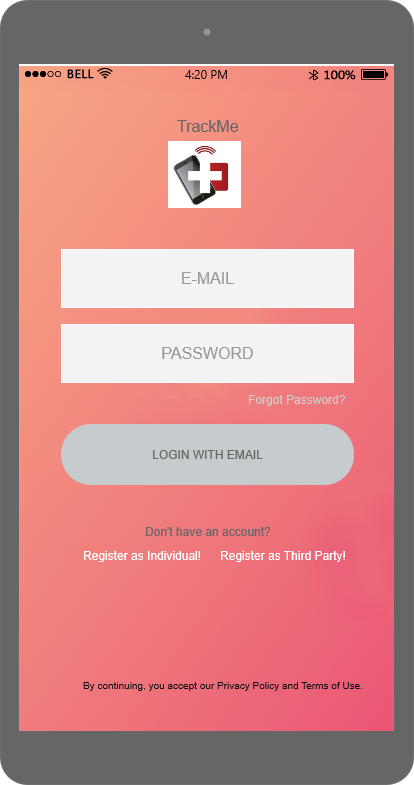
\includegraphics[width=4cm,height=7cm]		{./RASD_Mockups/1_Login.png}
      	\caption{Login for TrackMe}
        \label{TrackMe_login}
	 \end{subfigure}
\end{figure}
This is the login page where a user of type individual or third party can login by entering their credentials. If a user is new then they can register as individual or third party depending on their category.
\newline\newline\newline\newline
\textbf{Data4Help}
\newline\qquad{1. User Type: Individual}

\begin{figure}[H]
	\centering
	\begin{subfigure}[b]{0.4\textwidth}	
		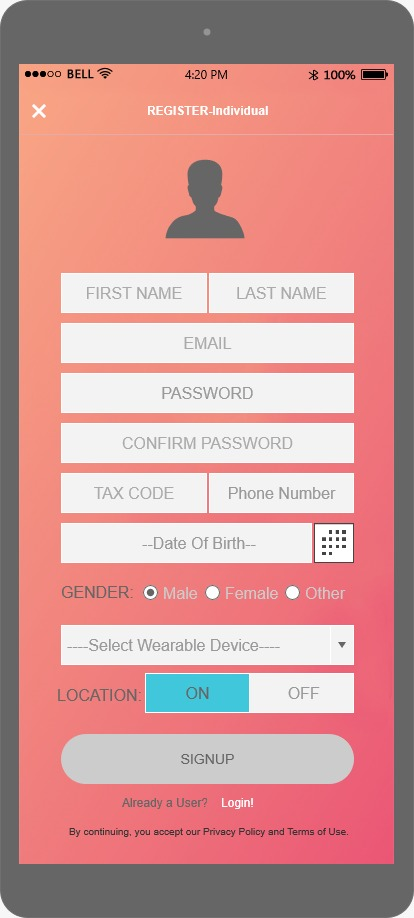
\includegraphics[width=4cm,height=7cm]		{./RASD_Mockups/2_I-Register.jpeg}
      	\caption{Registration for individuals}
        \label{TrackMe_register1}
	 \end{subfigure}
\end{figure}

The individual can check their vitals, and get to know about the third parties accessing their data and can receive the request of the third party which they can accept/reject when the third party asks the data about a specific individual.

\begin{figure}[H]
	\centering
	\begin{subfigure}[b]{0.3\textwidth}	
		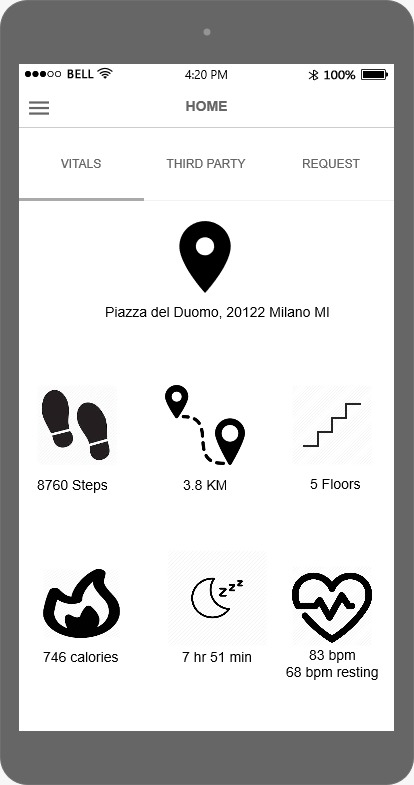
\includegraphics[width=4cm,height=7cm]		{./RASD_Mockups/3_I-Home.jpeg}
      	\caption{Individual Checks Vitals}
        \label{TrackMe_vitals}
	 \end{subfigure}
     \begin{subfigure}[b]{0.3\textwidth}	
		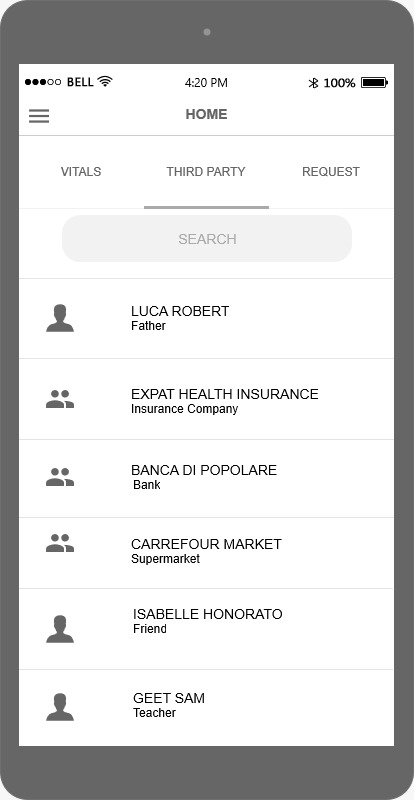
\includegraphics[width=4cm,height=7cm]		{./RASD_Mockups/4_I-DetailsOfThirdParty.jpeg}
      	\caption{Third party accessing individual's data}
        \label{TrackMe_3party}
	 \end{subfigure}
     \begin{subfigure}[b]{0.3\textwidth}	
		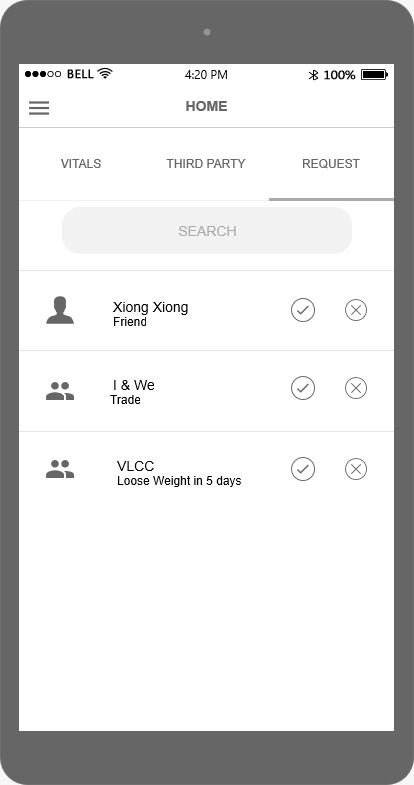
\includegraphics[width=4cm,height=7cm]		{./RASD_Mockups/5_I-Request.jpeg}
      	\caption{Accept/Reject access request}
        \label{TrackMe_acerej}
	 \end{subfigure}
\end{figure}

2. User Type: 3rd Party

\begin{figure}[H]
	\centering
	\begin{subfigure}[b]{0.4\textwidth}	
		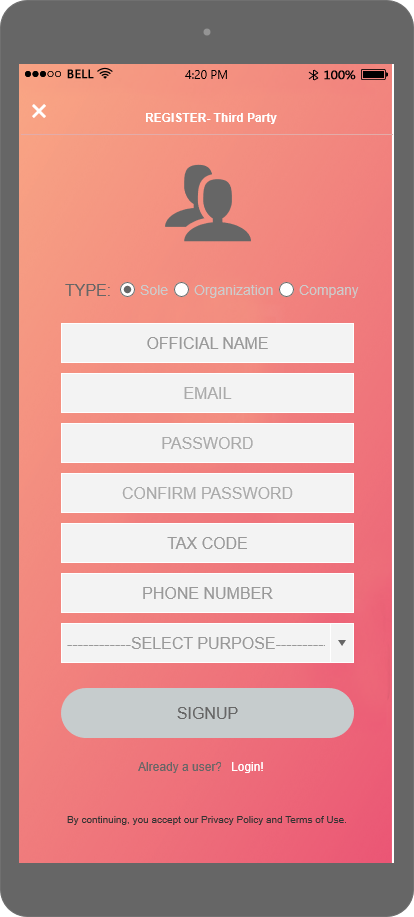
\includegraphics[width=4cm,height=7cm]		{./RASD_Mockups/2_T-Register.png}
      	\caption{Registration for Third Party}
        \label{TrackMe_register2}
	 \end{subfigure}
\end{figure}

Third party can check individual's or group of individual's data, make new requests for specific individual's data and group of individual's data, and view the status of earlier requests made to know whether they are requested, accepted or pending.

\begin{figure}[H]
	\centering
	\begin{subfigure}[b]{0.4\textwidth}	
		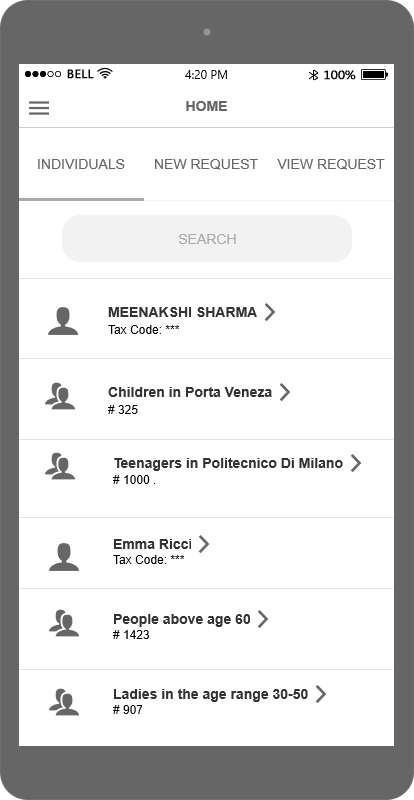
\includegraphics[width=4cm,height=7cm]		{./RASD_Mockups/3_T-Home.png}
      	\caption{Access individual's data}
        \label{TrackMe_data}
	 \end{subfigure}
     \begin{subfigure}[b]{0.4\textwidth}	
		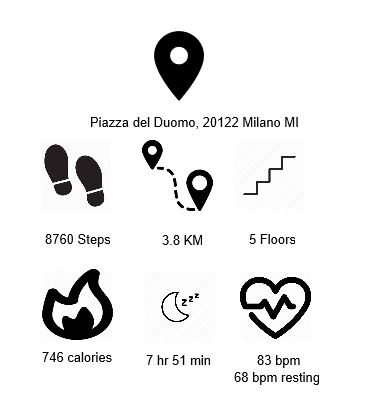
\includegraphics[width=\textwidth]		{./RASD_Mockups/3_T_popup.jpg}
      	\caption{This Popup appears on the screen on clicking on specific individual's list and for group of individuals another list of all individuals appears with their vitals.}
        \label{TrackMe_popup}
	 \end{subfigure}
\end{figure}

\begin{figure}[H]
	\centering
     \begin{subfigure}[b]{0.4\textwidth}	
		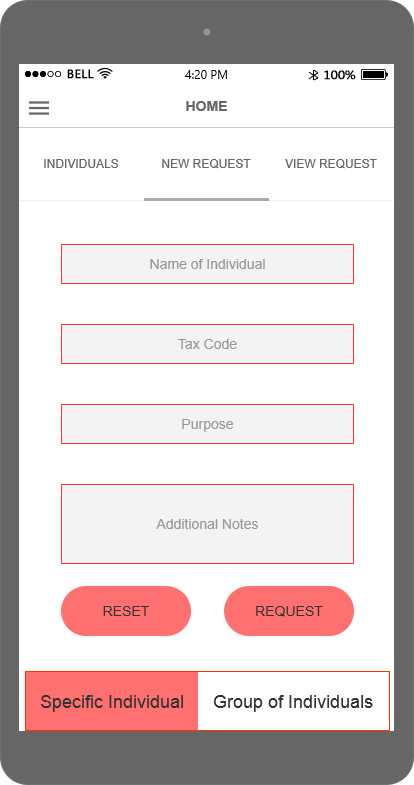
\includegraphics[width=4cm,height=7cm]		{./RASD_Mockups/4_T_1-NewRequest.png}
      	\caption{Make new request for individual}
        \label{TrackMe_reqind}
	 \end{subfigure}
     \begin{subfigure}[b]{0.4\textwidth}	
		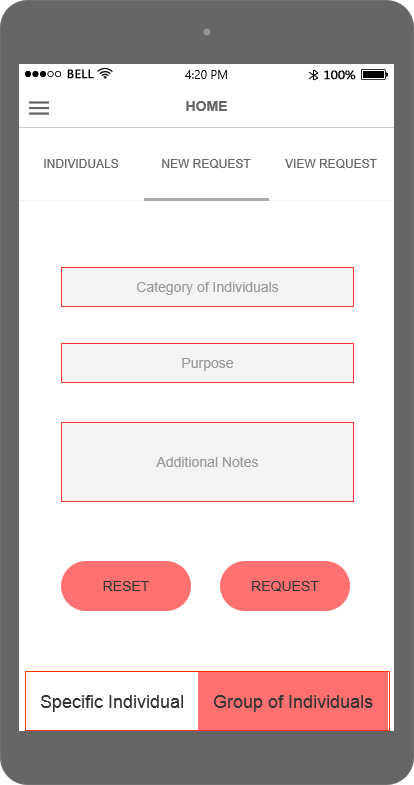
\includegraphics[width=4cm,height=7cm]		{./RASD_Mockups/4_T_2-NewRequest.png}
      	\caption{Make new request for Group of Individuals}
        \label{TrackMe_reqgroup}
	 \end{subfigure}
     \begin{subfigure}[b]{0.4\textwidth}	
		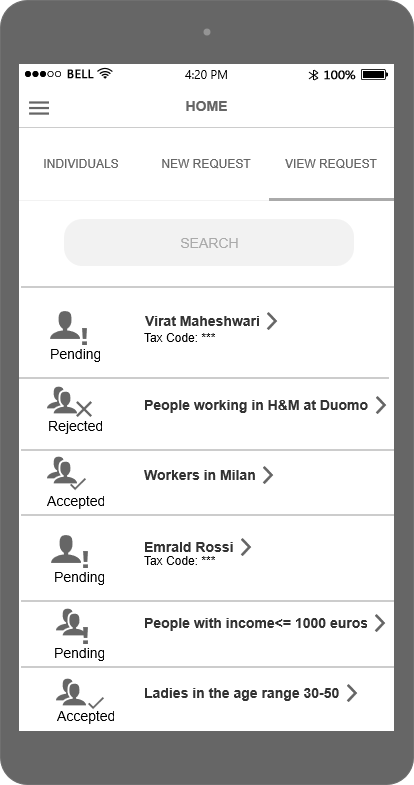
\includegraphics[width=4cm,height=7cm]		{./RASD_Mockups/5_T-ViewRequest.png}
      	\caption{View Requests}
        \label{TrackMe_viewreq}
	 \end{subfigure}
\end{figure}
.
\newline\newline\newline\newline\newline\newline\newline\newline
\textbf{Menu}
\newline
This includes all the extra features which is offered to the users. The menu remains same for both type of users: individual or third party.

\begin{figure}[H]
	\centering
	\begin{subfigure}[b]{0.4\textwidth}	
		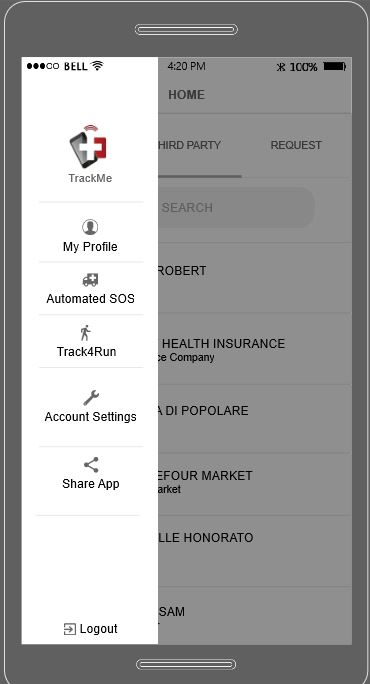
\includegraphics[width=4cm,height=7cm]		{./RASD_Mockups/6_Menu.JPG}
      	\caption{Menu}
        \label{TrackMe_Menu}
	 \end{subfigure}
\end{figure}

Menu-1. My Profile\newline
User can update their data in MyProfile section.

\begin{figure}[H]
	\centering
	\begin{subfigure}[b]{0.4\textwidth}	
		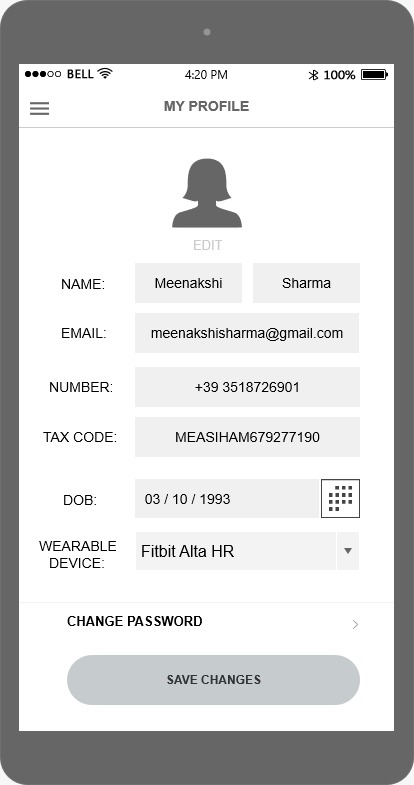
\includegraphics[width=4cm,height=7cm]		{./RASD_Mockups/7_I-MyProfile.jpeg}
      	\caption{Individual-MyProfile}
        \label{TrackMe_indpro}
	 \end{subfigure}
     \begin{subfigure}[b]{0.4\textwidth}	
		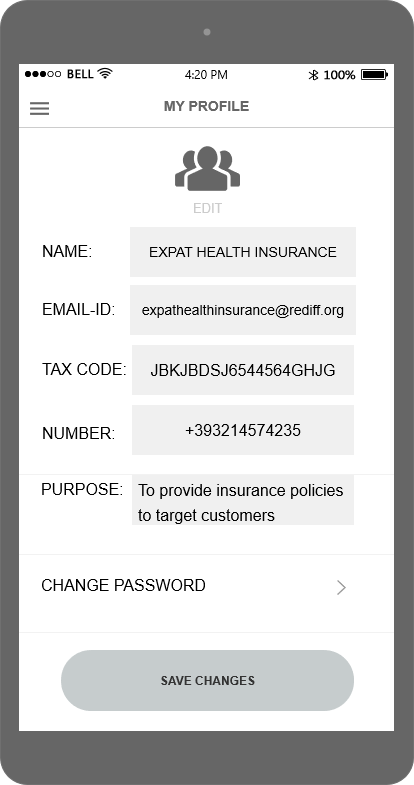
\includegraphics[width=4cm,height=7cm]		{./RASD_Mockups/7_T-MyProfile.png}
      	\caption{3rd Party-MyProfile}
        \label{TrackMe_3ppro}
	 \end{subfigure}
\end{figure}

.\newline\newline
Menu-2. AutomatedSOS\newline
This is only for individuals .\newline If they have not registered tot his service then they will be directed to the payment page where they can pay and register for the service.\newline If they have registered to this service, then they see a map with nearby hospitals and pharmacies.\newline In case of emergencies, they can track ambulance in the map.

\begin{figure}[H]
	\centering
	\begin{subfigure}[b]{0.4\textwidth}	
		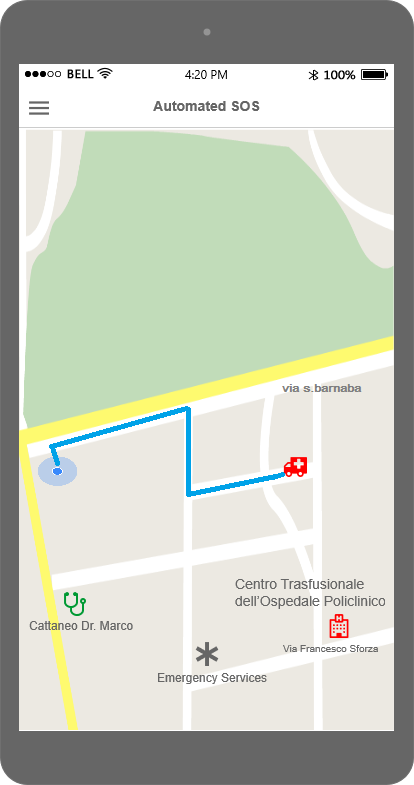
\includegraphics[width=4cm,height=7cm]		{./RASD_Mockups/8_I-AutomatedSOS.png}
      	\caption{AutomatedSOS}
        \label{TrackMe_AutomatedSOS}
	 \end{subfigure}
\end{figure}

Menu-3. Track4Run\newline
This service is for both the users, individual and third party.\newline If the user has not upgraded to this service, then for individual who can be an athlete or a spectator and the third party who can be a spectator will be directed to a payment page to pay and use the service.\newline The third party organizer who has not registered will be directed to a form and then a payment page. The organizer defines the path, theme of race and other details of the race in the form.\newline If the user has registered, then they will see a live map with all the position of the athletes.

\begin{figure}[H]
	\centering
	\begin{subfigure}[b]{0.4\textwidth}	
		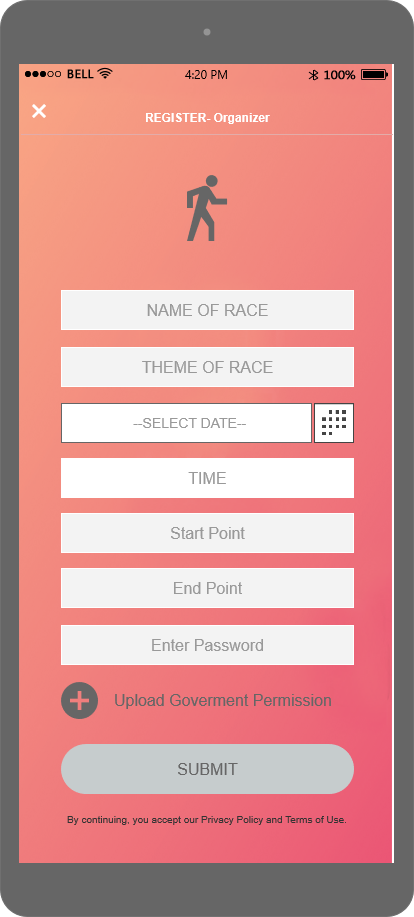
\includegraphics[width=4cm,height=7cm]		{./RASD_Mockups/9_T-Oragnizer.png}
      	\caption{Organizer form}
        \label{TrackMe_org}
	 \end{subfigure}
     \begin{subfigure}[b]{0.4\textwidth}	
		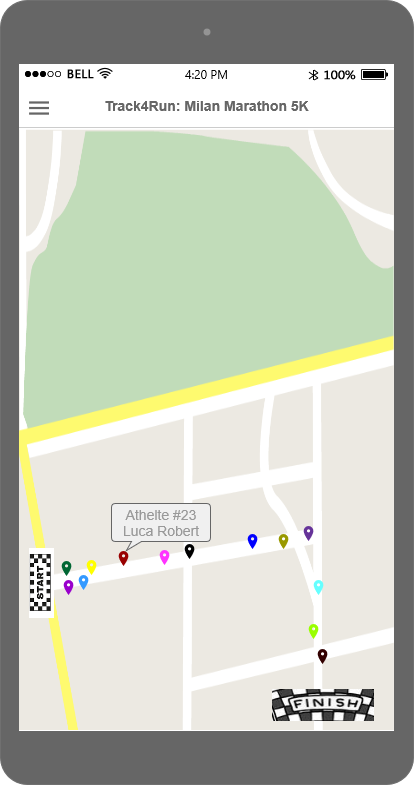
\includegraphics[width=4cm,height=7cm]		{./RASD_Mockups/9-Track4Run.png}
      	\caption{Track4Run}
        \label{TrackMe_Track4Run}
	 \end{subfigure}
\end{figure}

\textbf{Mobile Application for Ambulance Drivers}
This is an application made explicitly for Ambulance where they receive request in form of push notification and they accept it and the first driver to accept is navigates to the individual's location.

\begin{figure}[H]
	\centering
	\begin{subfigure}[b]{0.4\textwidth}	
		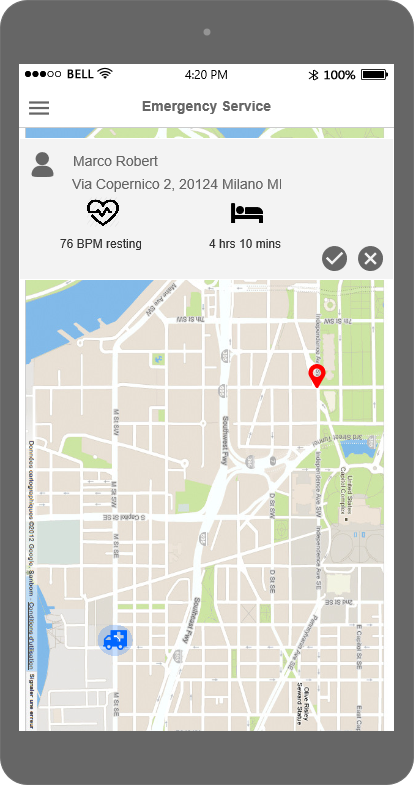
\includegraphics[width=4cm,height=7cm]		{./RASD_Mockups/1-Ambulance.png}
      	\caption{Accept Request}
        \label{TrackMe_ambulance}
	 \end{subfigure}
     \begin{subfigure}[b]{0.4\textwidth}	
		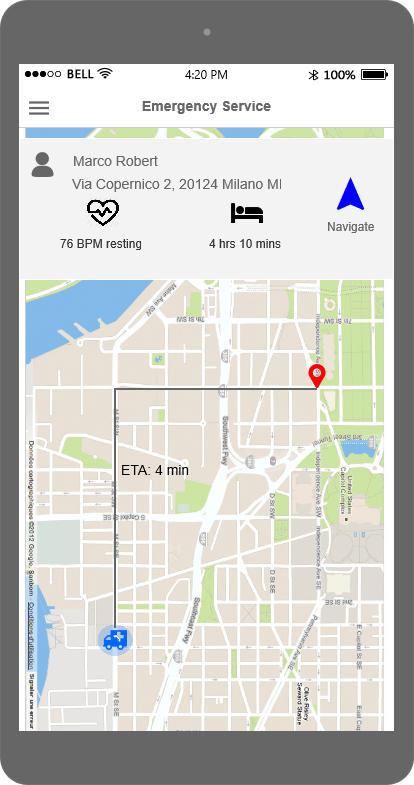
\includegraphics[width=4cm,height=7cm]		{./RASD_Mockups/2-Ambulance.png}
      	\caption{Navigate}
        \label{TrackMe_navigate}
	 \end{subfigure}
\end{figure}
.\newline\newline

\subsection{Software Interfaces}
\begin{enumerate}
\item \textbf{Data4Help API}
\newline \qquad TrackMe extracts location and health of the individual from the API of the   wearable device and stores it in a database. An API of the database is created which is provided to the other services of TrackMe. This information is used for many purposes. “AutomatedSOS” and “Track4Run” uses the API of the “Data4Help” in order to provide their service. Both the services exploit the services of “Data4Help”. “AutomatedSOS” uses the API to monitor the health status of elderly people and help them by providing an ambulance. “Track4Run” uses the API to extract the location and health of individuals registered as athletes. The location will be displayed to all the users and the health status of athletes will be monitored by the third party organizers.
\item \textbf{Ambulance Application}
\newline\qquad TrackMe develops an application for all the ambulance drivers associated with major Hospitals in the city of Milan. The application fetches the details and location of all the ambulance driver. When the health status of an subscribed individual is below a threshold value, the software sends a push notification to the nearby ambulance drivers phone with the details and location of the individual. Once an ambulance driver accept the request, the software removes the alert message from the application. The driver can navigate to the location of the individual in need of emergency using the map provided in the application.
\item \textbf{City Maps}
\newline\qquad We will be using Google Maps API to facilitate the location monitoring for third party services and insertion of race location in Track4Run and race visualization.
\end{enumerate}
.\newline\newline\newline\newline\newline\newline\newline
\subsection{Communication Interface}
The TrackMe application provides the Data4Help API which is used by the third party after validating for accessing individual's details and Track4Run for accessing the location of athletes. It also provides the details to the ambulance application API to use Automated SOS. All the external API's like Emergency Service API, Wearable Device API and Google Map API are connected as they provide information.
\begin{figure}[H]
	\centering	
		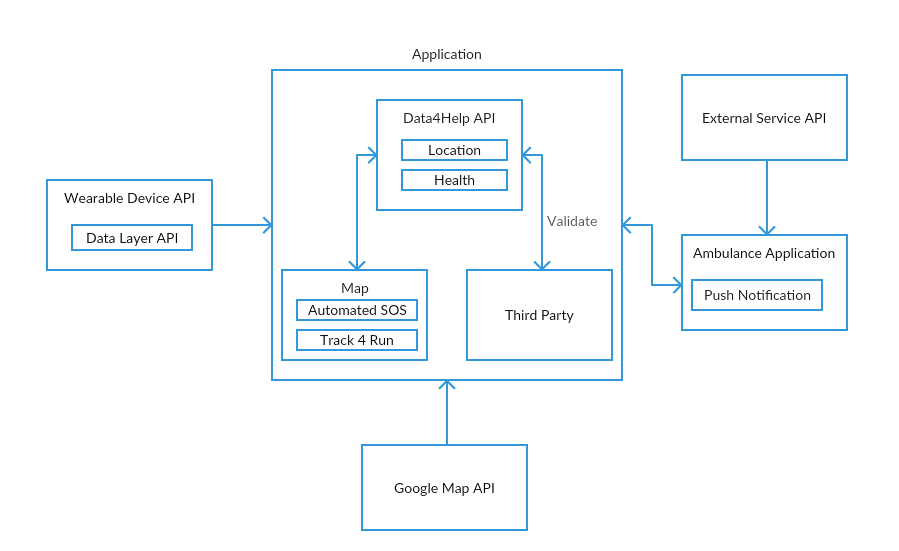
\includegraphics[width=\linewidth]		{./RASD_Diagrams/CommunicationInterface.png}
      	\caption{Communication Interface}
        \label{TrackMe_comint}
\end{figure}

\section{Functional requirements}
In order to fulfill the goals, with all the domain properties and assumption, listed in the above section of the document, the following requirements can be derived. Each goal has its own set of requirement and they are mentioned below.\newline

\begin{itemize}

\item\textbf{[G1]} Providing a list of the wearable devices that an individual can choose from.

\begin{itemize}
\item\textbf{[R1]} The location and the health status of an individual should be fetched by the wearable device API.
\item\textbf{[R2]} Individual should be able to update their wearable device.
\item\textbf{[A3]} Vitals taken from the wearable devices are reliable.
\item\textbf{[A5]} GPS provides accurate positions and incase the signal is lost, last active location would be considered.
\item\textbf{[C1]} Only a few wearable devices are compatible with application.\newline
\end{itemize}

\item\textbf{[G2]} Expedite the request made by the 3rd party to an individual to access their details.

\begin{itemize}
\item\textbf{[R3]} Individual must be able to view the name and the purpose/relationship of the 3rd party who requested the data.
\item\textbf{[R4]} The details of all the 3rd party accessing the individual’s data must be visible.\newline
\end{itemize}

\item\textbf{[G3]} Provides an interface for an individual to analyze the request made by the 3rd party.

\begin{itemize}
\item\textbf{[R5]} The system must provide a choice to an Individual to accept or reject the request of the 3rd party.\newline
\end{itemize}
\item\textbf{[G4]} Validating the request made by the 3rd party to provide the details of a group of individuals.
\begin{itemize}
\item\textbf{[R6]} The system checks whether the request made by the 3rd party is of more than 1000 Individuals.
\item\textbf{[R7]} The details of the group of individual must be displayed in a list.
\item\textbf{[R8]} The details of an individual should be displayed in a pop up dialog.\newline
\end{itemize}

\item\textbf{[G5]} Quick access of the data to the 3rd party once the request is approved.

\begin{itemize}
\item\textbf{[R9]} Allow a 3rd party to an instant access of the previously saved data after it is approved.
\item\textbf{[R10]} 3rd party must view all the updated data of the individual. \newline
\end{itemize}

\item\textbf{[G6]} Immediate update of the data once an individual updates their own details.

\begin{itemize}
\item\textbf{[R11]} An individual should be able to update all their details.
\item\textbf{[R12]} Allow a 3rd party to access the new data as soon as the individual updates it.\newline
\item \textbf{[A12]} All details entered by the users are genuine.
\end{itemize}

\item\textbf{[G7]}  Provides an upgradation to the new services, Automated SOS or Track4Run.

\begin{itemize}
\item\textbf{[R13]} They system shall redirect to a payment gateway once a new service is selected.
\item\textbf{[D17]} Payment Details are genuine and transactions are processed positively.\newline
\end{itemize}

\item\textbf{[G8]} Monitoring the health status of the subscribed individual to the Automated SOS service.

\begin{itemize}
\item\textbf{[R14]} The system must compare the vitals of the individual with the Threshold value of health.
\item\textbf{[R15]} If the system detect that the health status of the individual is below the threshold value, send an alert to a nearby Ambulance with the location and details of the subscribed user.
\item\textbf{[R16]} To ensure the reaction time of less than 5 seconds, Push notification must be send to the ambulance driver application.
\item\textbf{[C2]}The services provided by the application are limited to the citizens of Milan.
\item \textbf{[A6]} We assume that a certain number of hospitals are registered to with TrackMe which provide Ambulance services.
\item \textbf{[A7]} We assume there are no network issues between the time we sent a message and the drivers receive it.
\item\textbf{[C3]}This application is connected only with the major hospitals in Milan for Ambulance services\newline
\end{itemize}

\item\textbf{[G9]]}  Develops an interface to organize a race for the subscribed 3rd party to the Track4Run service.

\begin{itemize}
\item\textbf{[R17]} An organizer get to add an event only after he/she/they register for Track4Run service in the application.
\item\textbf{[R18]} Registration involves, providing his/her email, phone number for verification and a unique user name.
\item\textbf{[R19]} An event can be added with the following details like event name, time and location of the event.
\item\textbf{[A15]} The payment details given are genuine and transactions are processed positively.
\item\textbf{[A8]} Organizers can keep a maximum limit of the participants who can join the event.\newline
\end{itemize}

\item\textbf{[G10]} Give access to the details of the race once an individual participate in it.

\begin{itemize}
\item\textbf{[R20]} Participant has to register for the event.
\item\textbf{[R21]} While registering, his/her details like name, age and wearable device to be used are requested.
\item\textbf{[A10]} All athletes have their own wearable device.\newline
\end{itemize}

\item\textbf{[G11]} Live visualization of the race .

\begin{itemize}
\item\textbf{[R22]} A spectator upon registration can view the live event.
\item\textbf{[R23]} He/She also gets to choose subscribe for upcoming events.
\item\textbf{[A10]} All athletes have their own wearable device.\newline
\end{itemize}

\end{itemize}


\section{UML Modeling}
\subsection{Use Case Diagrams}
\begin{figure}[H]
	\begin{center}
		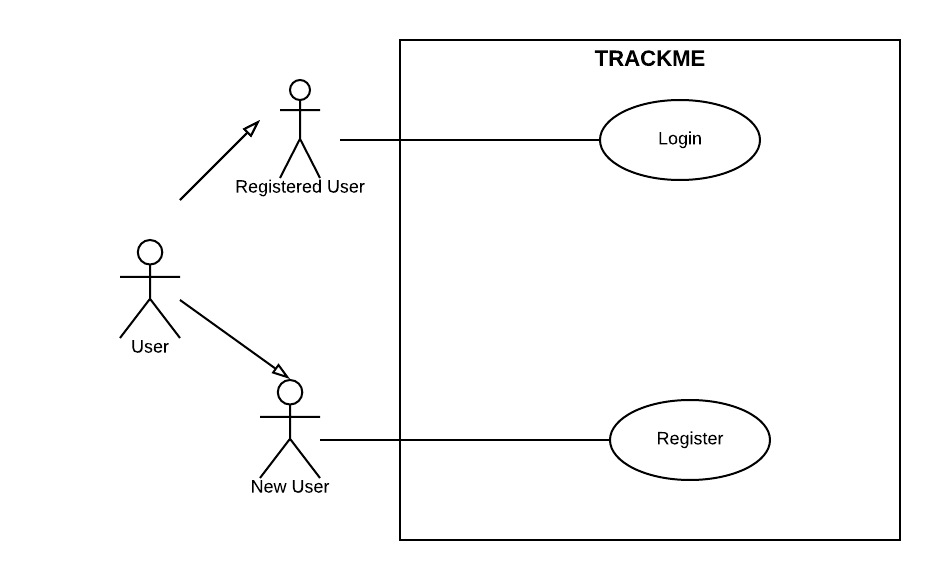
\includegraphics[width=\textwidth]{./RASD_Diagrams/UseCase_TrackMe.png}
      	\caption{Use case for TrackMe application}
        \label{TrackMe_usecase}
	\end{center}
\end{figure}


\begin{figure}[H]
	\begin{center}
		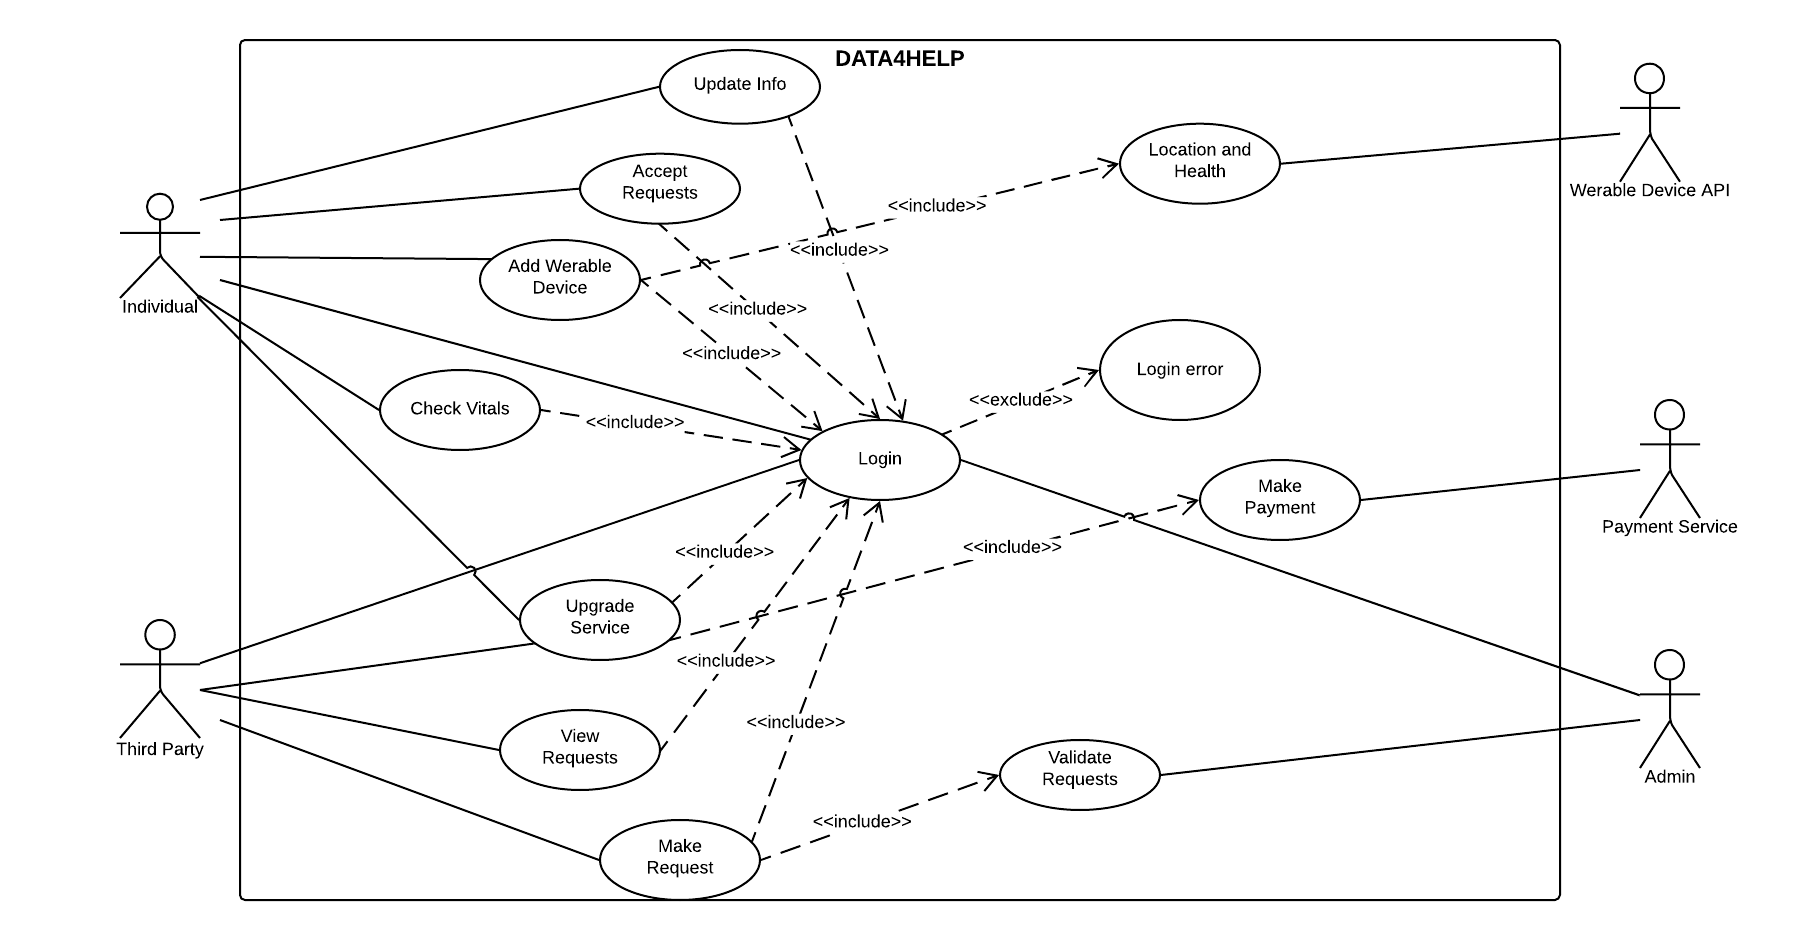
\includegraphics[width=\textwidth]{./RASD_Diagrams/UseCase_Data4Help.png}
        \caption{Use case for Data4help}
        \label{Data4help}
	\end{center}
\end{figure}

\begin{figure}[H]
	\begin{center}
		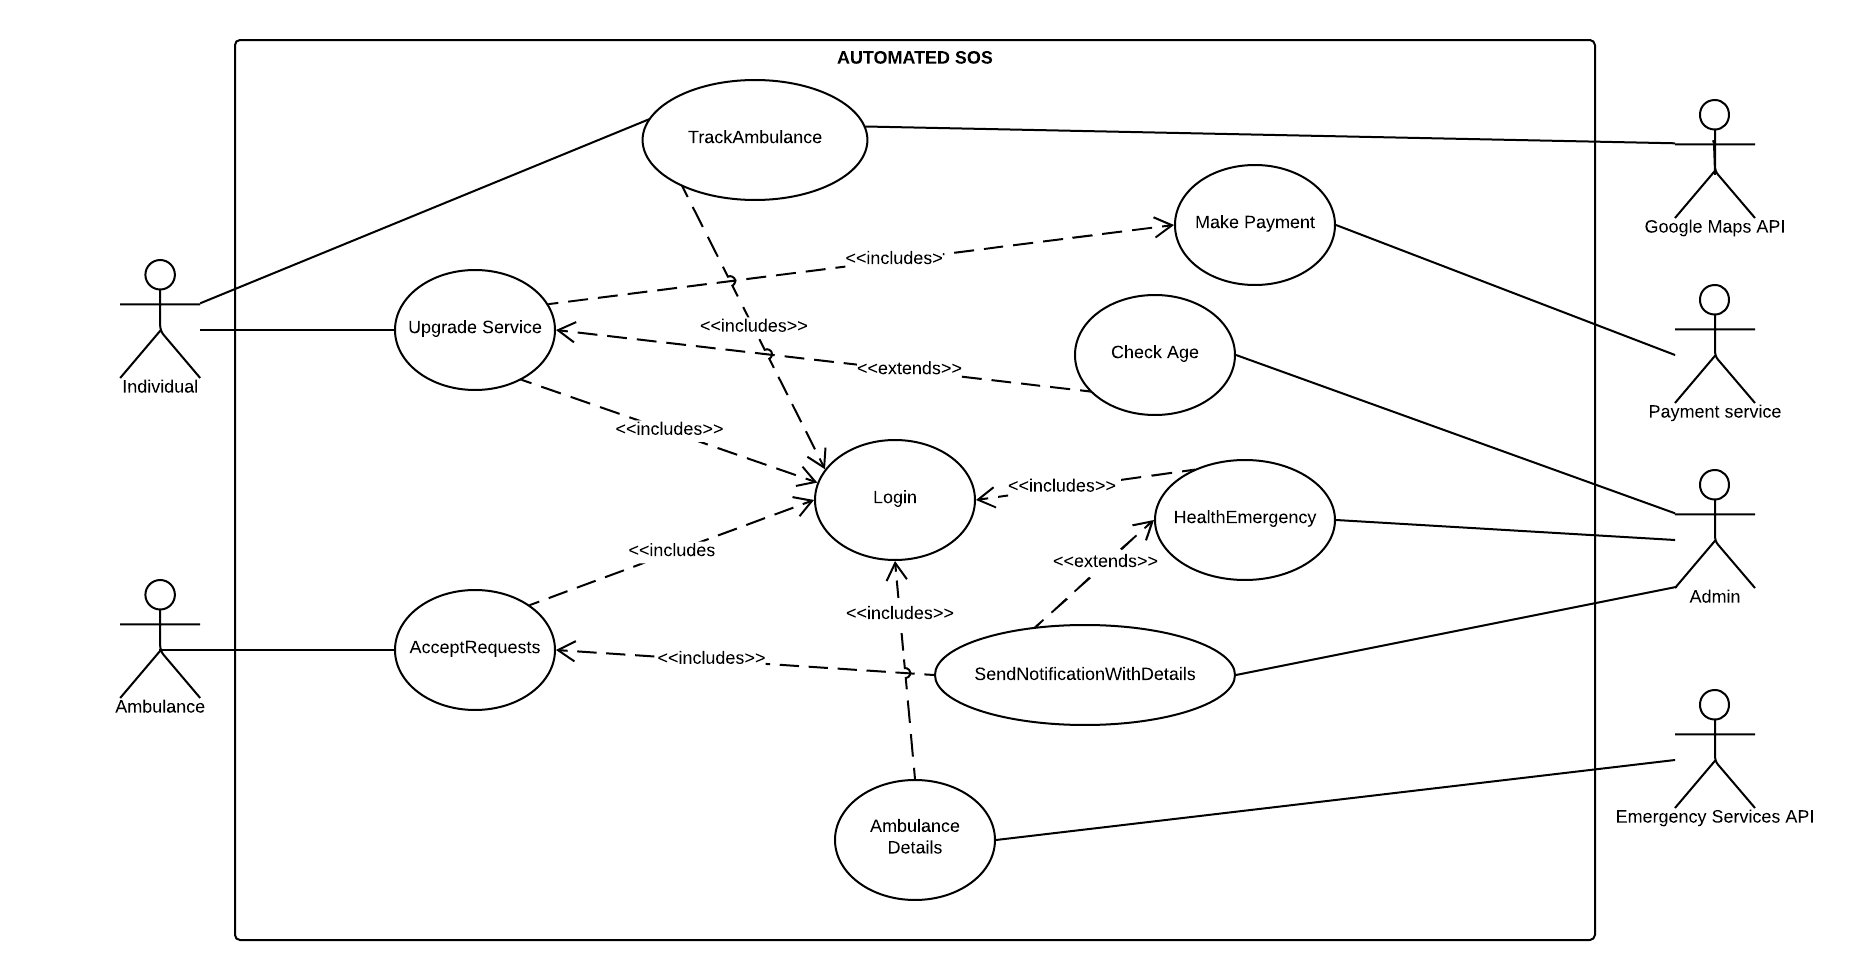
\includegraphics[width=\textwidth]{./RASD_Diagrams/UseCase_AutomatedSOS.png}
        \caption{Use case for Automated SOS}
        \label{track4run}
	\end{center}
\end{figure}

\begin{figure}[H]
	\begin{center}
		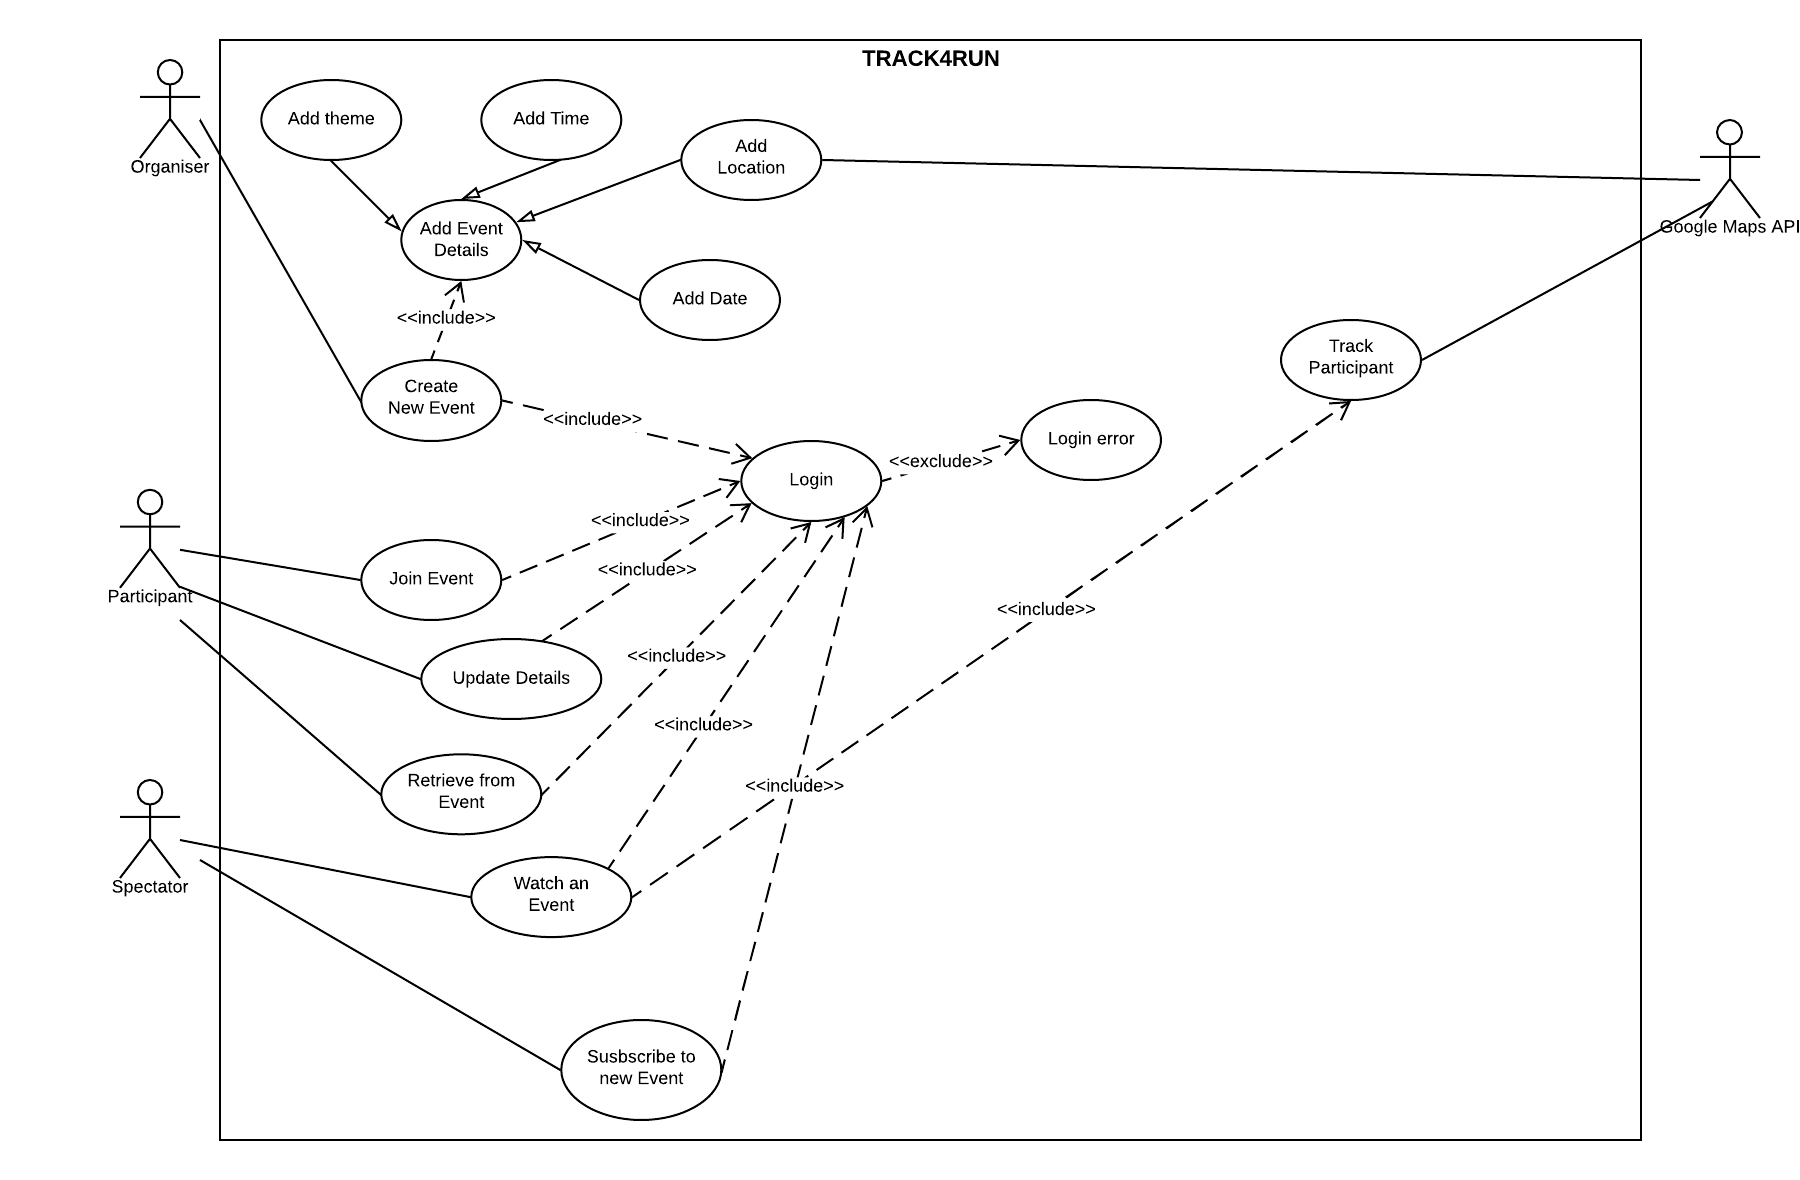
\includegraphics[width=\textwidth]{./RASD_Diagrams/UseCase_Track4Run.png}
        \caption{Use case for track4run}
        \label{track4run}
	\end{center}
\end{figure}


%================================Login===============================%
\begin{table}[H]
\begin{center}
\begin{tabular}{| l | p{0.75\textwidth} |}
\hline
Name & Login \\
\hline
Actors & Registered Users(Individual or Third Party)
\\
\hline
Entry condition & \begin{enumerate}
\item The user has successfully logged into the system
\item The user is not logged into the system yet
\end{enumerate}  \\
\hline
Event Flow & \begin{enumerate}
	\item The user opens the welcome page of the application and forwards to sign in
	\item He/She provides the valid credentials for login, say user name and password.
	\item User gets to authenticate into the application incase his credentials are valid.
    \item His/Her dashboard shows the services to which he/she is registered with.
	
\end{enumerate}
\\
\hline
Exit Conditions & The user successfully redirects to the dashboard. \\
\hline
Exception & 
The credentials provided by the user are invalid, in this case a login error message is shown and allows the user to input the username and password again.\\
\hline
\end{tabular}
\end{center}
\caption{Use case for Login.}
\label{usecase-login}
\end{table}

%========================Adding a Wearable device==========================%

\begin{table}[H]
\begin{tabular}{| l | p{0.75\textwidth} |}
\hline
Name & Add wearable Device\\
\hline
Actors & Individual\\
\hline
Entry condition & \begin{enumerate}
  \item The individual has successfully logged into the system.
  \item The individual has a wearable device supported by trackme
\end{enumerate}  \\
\hline
Event Flow & \begin{enumerate}
  \item Selects the add new wearable device button.
  \item Select the compatible device name from the given options.
  \item Connection successful.
\end{enumerate}
\\
\hline
Exit Conditions & The individual successfully connects to the device and navigates back to dashboard. \\
\hline
Exception & 
All devices are not compatible with TrackMe application. The user selects there wearable device among the list of compatible device from Dropdown. An error message is shown in case of connection problems.\\
\hline
\end{tabular}
\caption{Use case for adding a new wearable device.}
\label{usecase-adddevice}
\end{table}

%==========================Accept/Reject Requests=========================%


\begin{table}[H]
\begin{tabular}{| l | p{0.75\textwidth} |}
\hline
Name & Accept or Reject Requests\\
\hline
Actors & Individual\\
\hline
Entry condition & No entry conditions\\
\hline
Event Flow & \begin{enumerate}
\item The individual can see those requests made by a third party for specific individual health vitals or location.
\item He/She gets to accept or reject the requests.
\item The status of the request on the individual's dashboard will be updated with the corresponding response
\end{enumerate}
\\
\hline
Exit Conditions & The individual successfully redirects to the dashboard.\\
\hline
\end{tabular}
\caption{Use case for Accept or reject requests.}
\label{usecase-accorrejrequests}
\end{table}

%============================Update Info================================%
\begin{table}[H]
\begin{tabular}{| l | p{0.75\textwidth} |}
\hline
Name & Update Info\\
\hline
Actors & User\\
\hline
Entry condition & No entry conditions\\
\hline
Event Flow & \begin{enumerate}
\item Upon clicking on the update Info button, user gets to change the information given earlier.
\item Once he makes the corresponding changes, user can save it or cancel it.
\item Upon saving changes will be updated.
\end{enumerate}
\\
\hline
Exit Conditions & 
The user successfully redirects to the dashboard.\\
\hline
Exceptions & Upon providing invalid details, the user will be requested to enter the details again. Upon canceling the changes made would be lost.\\
\hline
\end{tabular}
\caption{Use case for Update Info requests.}
\label{usecase-taxiavailability}
\end{table}

%==========================Make Requests===============================================%
\begin{table}[H]
\begin{tabular}{| l | p{0.75\textwidth} |}
\hline
Name & Make Requests\\
\hline
Actors & Third Party\\
\hline
Entry condition & \begin{enumerate}
\item The third party is successfully logged into the system as a third party.
\item The third party needs needs health and location data of individuals or a group of individuals.
\end{enumerate}\\
\hline
Event Flow & \begin{enumerate}
\item The third party clicks the Make Requests button.
\item He/She/They are requested to select the type of request- individual or group of individuals.
\item Enter the valid reason for the request
\item Click the submit button.
\item The request is then validated by Trackme or individual according to the category.
\end{enumerate}
\\
\hline
Exit Conditions & The user successfully redirects to the dashboard once the requests is made.\\
\hline
\end{tabular}
\caption{Use case for Making requests.}
\label{usecase-Making-requests}
\end{table}

%====================================View Requests===================================%

\begin{table}[H]
\begin{tabular}{| l | p{0.75\textwidth} |}
\hline
Name & Check Status\\
\hline
Actors & Third Party\\
\hline
Entry condition & \begin{enumerate}
\item No entry conditions
\end{enumerate}\\
\hline
Event Flow & \begin{enumerate}
\item The Third Party clicks the Check status button.
\item The list of requests made by him/her is available with the status(approved or still waiting to be approved) of the requests
\end{enumerate}\\
\hline
Exit Conditions & The Third Party successfully navigates back.\\
\hline
Exceptions & Incase the Third Party has not made any requests a message stating “ No requests found” will be shown.\\
\hline
\end{tabular}
\caption{Use case for view requests.}
\label{usecase-view-requests}
\end{table}

%====================================Upgrade Service===================================%
\begin{table}[H]
\begin{tabular}{| l | p{0.75\textwidth} |}
\hline
Name & Upgrade Service\\
\hline
Actors & Third Party or Individual\\
\hline
Entry condition & The user needs to access a new service\\
\hline
Event Flow & \begin{enumerate}
\item The user clicks the service they want to upgrade.
\item Choose the duration for the service.
\item Directs to the payment page
\item Makes the payment and completes the transaction.
\end{enumerate}
\\
\hline
Exit Conditions & The user successfully redirects to the dashboard.\\
\hline
Exceptions & Transaction errors can happen, in that case he/she is asked to provide the credentials again and try. \\
\hline
\end{tabular}
\caption{Use case for Upgrade Service.}
\label{usecase-upgradeservice}
\end{table}

%==============================Validate Requests=======================================%

\begin{table}[H]
\begin{tabular}{| l | p{0.75\textwidth} |}
\hline
Name & Validate Requests\\
\hline
Actors & Admin\\
\hline
Assumptions & There are some requests made by the third party service.\\
\hline
Entry condition & No entry conditions\\
\hline
Event Flow & \begin{enumerate}
\item Checks for the latests requests and categorize them. 
\item Incase of requests for individuals the request is forwarded to the individual.
\item Incase of request for group of data, validity of reasons provided are checked. If the group of people requested for is greater than 1000, th request is accepted. 
\item Status of requests are updated.
\end{enumerate}
\\
\hline
Exit Conditions & None\\
\hline
Exceptions & If the requests are fake, then the requests are rejected. \\
\hline
\end{tabular}
\caption{Use case for Validate Requests.}
\label{usecase-validate-requests}
\end{table}
%==================================================================%
%               Automated SOS                                         %
%===================================================================%
%===================Send Notification to Ambulance Drivers=================================%
\begin{table}[H]
\begin{tabular}{| l | p{0.75\textwidth} |}
\hline
Name & Send Notification to Ambulance Drivers\\
\hline
Actors & Admin\\
\hline
Assumptions & The emergency health condition monitored is accurate as they are calculated on the basis of 3 readings.
\\
\hline
Entry condition & No entry conditions\\
\hline
Event Flow & \begin{enumerate}
\item Check for emergency condition of any individual.
\item Send push notification to all nearby ambulance drivers as soon as the emergency is encountered. The push notification guarantees a reaction time less than 5 seconds.
\item The push notification contains all the details of the individual.
\item The individual can also track the ambulance in their application's map.
\end{enumerate}
\\
\hline
Exit Conditions & None\\
\hline
Exceptions & None. \\
\hline
\end{tabular}
\caption{Use case for Send Push Notification.}
\label{usecase-push-notification}
\end{table}
%===================Accept individual request and navigate to their location=================================%
\begin{table}[H]
\begin{tabular}{| l | p{0.75\textwidth} |}
\hline
Name & Accept individual request and navigate to their location\\
\hline
Actors & Ambulance Driver\\
\hline
Assumptions &  The notification will be received by all nearby ambulance drivers and the first driver to accept the request will navigate to the individual's location.
\\
\hline
Entry condition & Receive a push notification and accept it.\\
\hline
Event Flow & \begin{enumerate}
\item The driver receives a push notification in the application for ambulance drivers.
\item They accept the request.
\item The first driver to accept the request navigates to individual's location with any emergency products if required.
\end{enumerate}
\\
\hline
Exit Conditions & Reject request\\
\hline
Exceptions & None. \\
\hline
\end{tabular}
\caption{Use case for Ambulance drivers accepting request.}
\label{usecase-ambulance-driver}
\end{table}
%==================================================================%
%               TRACK4RUN                                          %
%===================================================================%

%===================Create a New Event=================================%
\begin{table}[H]
\begin{tabular}{| l | p{0.75\textwidth} |}
\hline
Name & Create a new Event\\
\hline
Actors & Organizer\\
\hline
Assumptions & He/She needs to host a new event(race)\\
\hline
Entry condition & Must provide all event details and pay for organizing\\
\hline
Event Flow & \begin{enumerate}
\item Click on the create event Button
\item Enter the Details(Name, Location, Time, Reason)
\item Submit the details 
\end{enumerate}
\\
\hline
Exit Conditions & Event is successfully created and navigated to the dashboard\\
\hline
Exceptions & Incase the user gives an invalid location, he/she will be asked to re try again. Incase the location and time is already booked for another event a warning would be shown. \\
\hline
\end{tabular}
\caption{Use case for New Event/Race.}
\label{usecase-new-event/race}
\end{table}

%======================================Join Event=============================%

\begin{table}[H]
\begin{tabular}{| l | p{0.75\textwidth} |}
\hline
Name & Join Event\\
\hline
Actors & Participant\\
\hline
Assumptions & He/She needs to participate in an event\\
\hline
Entry condition & No entry conditions\\
\hline
Event Flow & \begin{enumerate}
\item He/She registers for an event 
\item Adds the required details which includes the wearable device,name, place etc.
\item Confirms the availability 
\item Submit the details
\end{enumerate}
\\
\hline
Exit Conditions & The Athlete successfully joins the event. \\
\hline
Exceptions & An error message would be generated incase the maximum limit for the participants have reached.\\
\hline
\end{tabular}
\caption{Use case for Joining an event/Race.}
\label{usecase-join-event/race}
\end{table}

%==================================Watch an event================================================%

\begin{table}[H]
\begin{tabular}{| l | p{0.75\textwidth} |}
\hline
Name & Watch an Event\\
\hline
Actors & Spectator\\
\hline
Entry condition & Should be logged in as a spectator\\
\hline
Event Flow & \begin{enumerate}
\item The user chooses the race which he wants to watch now.
\item Upon clicking a view, he/she can watch the race live.
\item He/She can navigate out whenever the user wants
\end{enumerate}
\\
\hline
Exit Conditions & Navigate back to the dashboard \\
\hline
Exceptions & Incase the user is not subscribed for any event, he/she won’t be able to see any. Incase the user has not made the payment, he/she won’t be able to watch the event. \\
\hline
\end{tabular}
\caption{Use case for watching an event/Race.}
\label{usecase-watch-event/race}
\end{table}


%+++++++++++++++++++++++++++++++++++++++++++++++++++++++++++++++++++++++++++++++++++++++++++++++++++++++%
%                                          SEQUENCE DIAGRAMS                                            %
%++++++++++++++++++++++++++++++++++++++++++++++++++++++++++++++++++++++++++++++++++++++++++++++++++++++++%
\subsection{Sequence Diagram}
1. Accept/Reject Third party requests:
\begin{figure}[H]
	\begin{center}
		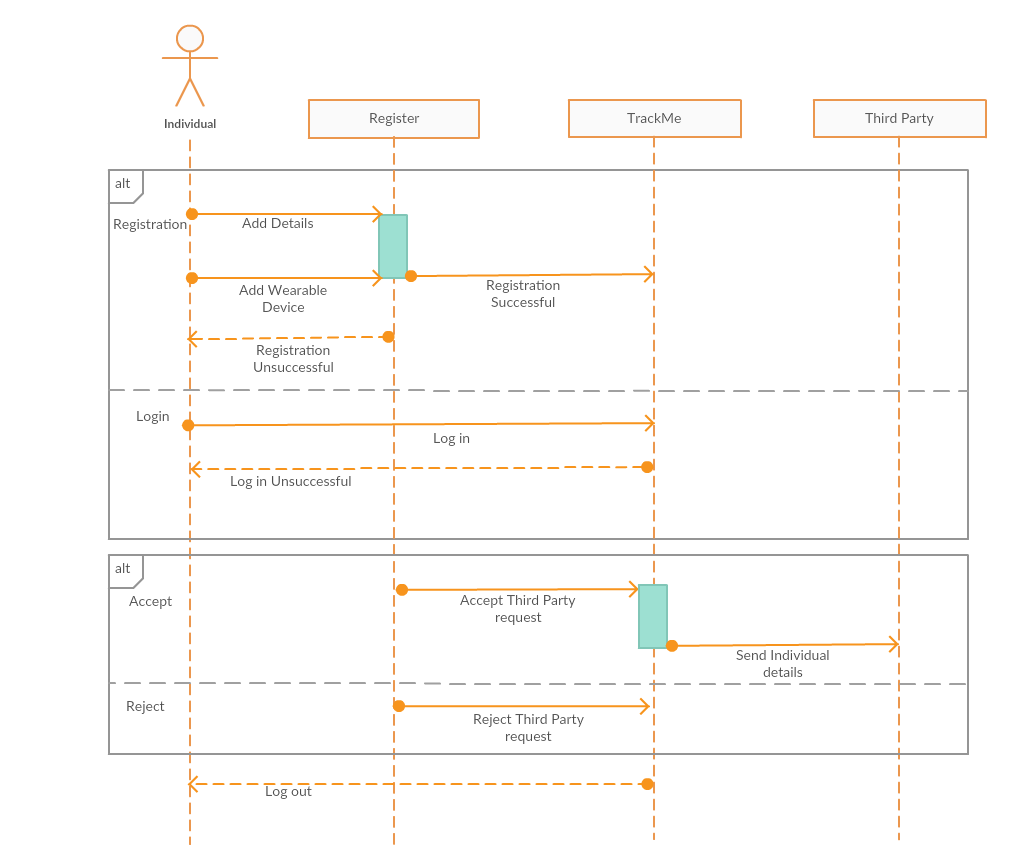
\includegraphics[width=\textwidth]{./RASD_Sequence/1__Individual.png}
      	\caption{Accept/Reject Third party requests.}
        \label{TrackMe_seq1}
	\end{center}
\end{figure}
.\newline\newline\newline\newline\newline\newline\newline\newline\newline\newline\newline
2. Third Party makes new request:
\begin{figure}[H]
	\begin{center}
		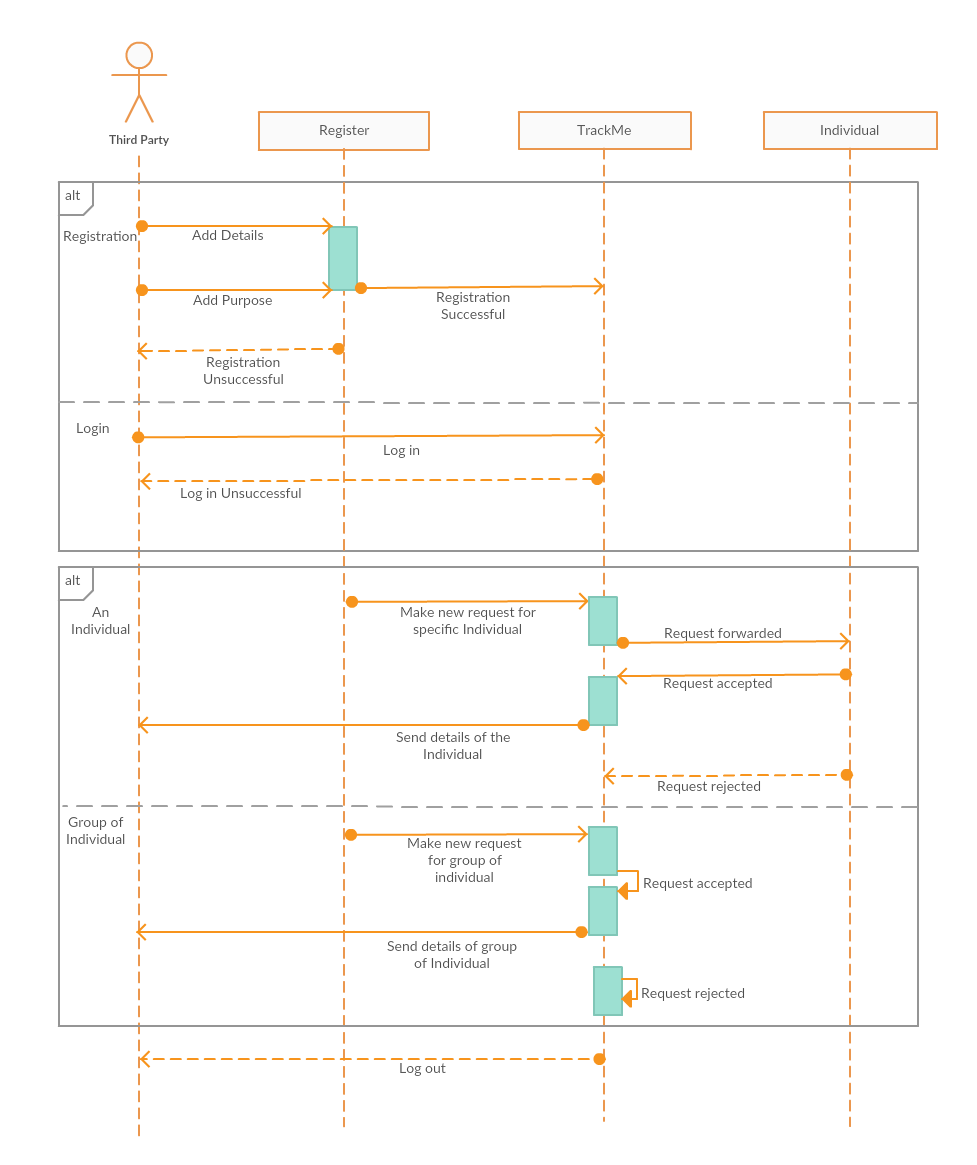
\includegraphics[width=\textwidth]{./RASD_Sequence/2__ThirdParty.png}
      	\caption{Third Party makes new request.}
        \label{TrackMe_seq2}
	\end{center}
\end{figure}
.\newline\newline
3. TrackMe validates request:
\begin{figure}[H]
	\begin{center}
		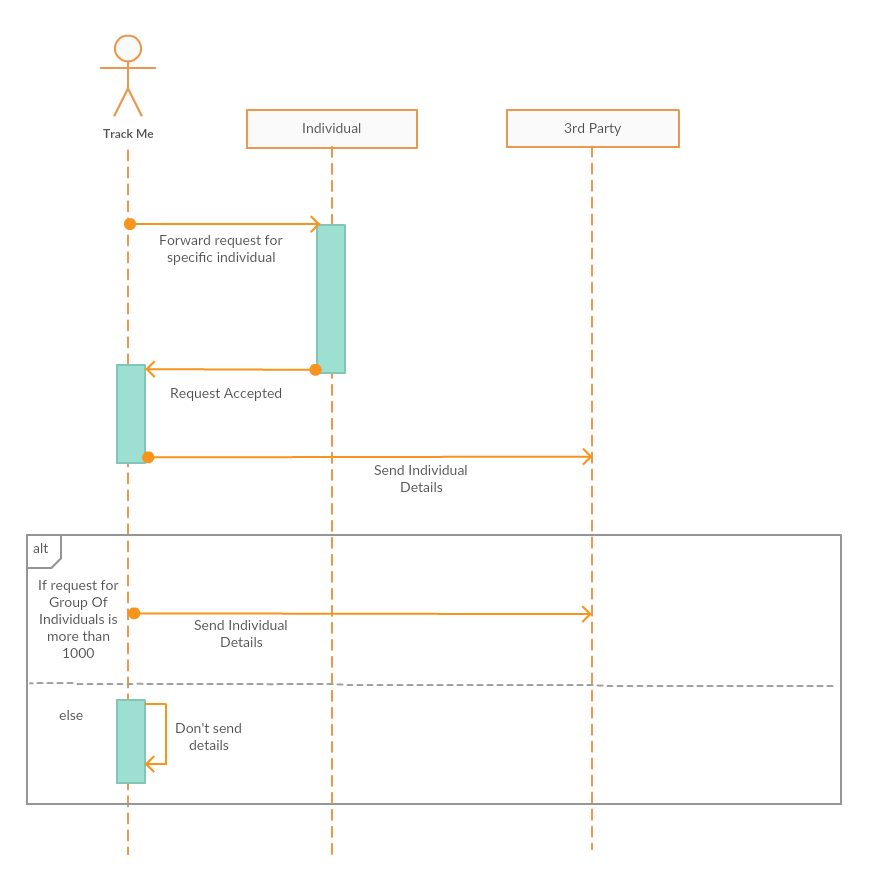
\includegraphics[width=\textwidth]{./RASD_Sequence/3__TrackMe.png}
      	\caption{TrackMe validates request.}
        \label{TrackMe_seq3}
	\end{center}
\end{figure}
.\newline\newline\newline\newline\newline\newline\newline\newline
4. Check vitals and send push notification:
\begin{figure}[H]
	\begin{center}
		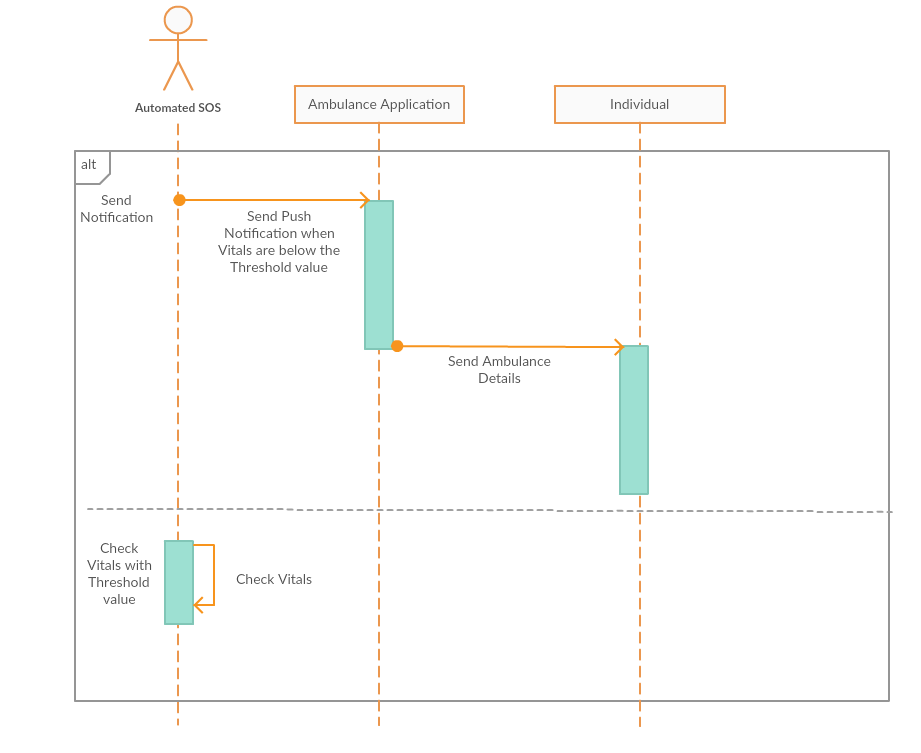
\includegraphics[width=\textwidth]{./RASD_Sequence/4_Automated_SOS.png}
      	\caption{Check vitals and send push notification.}
        \label{TrackMe_seq4}
	\end{center}
\end{figure}
.\newline\newline\newline\newline\newline\newline\newline\newline\newline\newline\newline\newline\newline
5. Ambulance Drivers accepts the request of push notifications and navigate to their location:
\begin{figure}[H]
	\begin{center}
		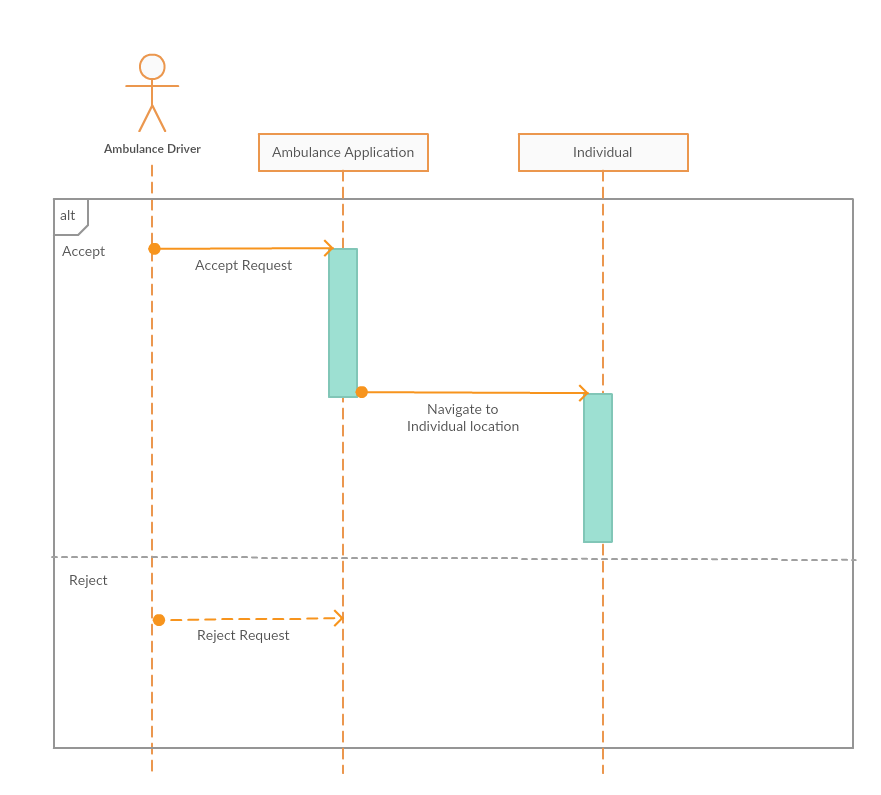
\includegraphics[width=\textwidth]{./RASD_Sequence/5_AmbulanceDriver.png}
      	\caption{Accept request of push notifications and Navigate to their location.}
        \label{TrackMe_seq5}
	\end{center}
\end{figure}
.\newline\newline\newline\newline\newline\newline\newline\newline\newline
6.Organizer adds race and defines path:
\begin{figure}[H]
	\begin{center}
		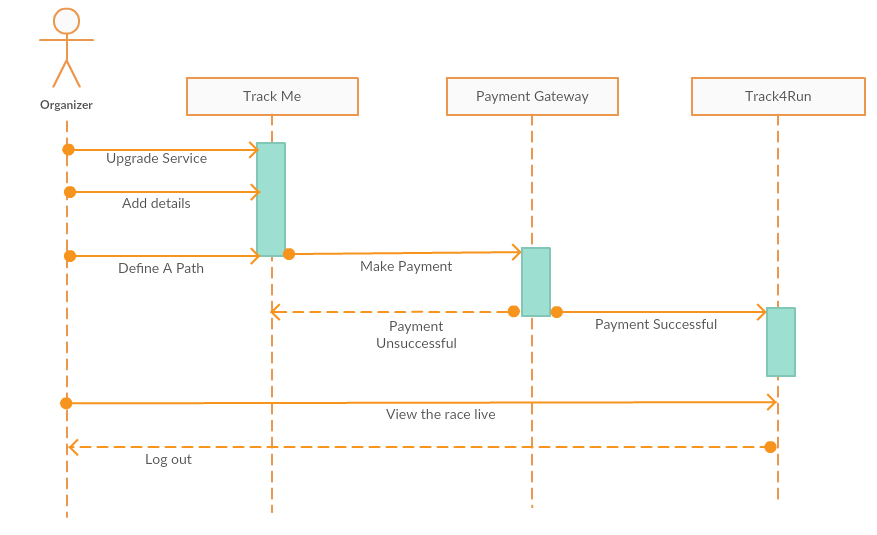
\includegraphics[width=\textwidth]{./RASD_Sequence/6_Organizer.png}
      	\caption{Organizer adds race and defines path.}
        \label{TrackMe_seq6}
	\end{center}
\end{figure}
.\newline\newline\newline\newline\newline\newline\newline\newline\newline\newline\newline\newline\newline\newline\newline\newline\newline\newline\newline
7. Athletes participate and Spectators view the race:
\begin{figure}[H]
	\begin{center}
		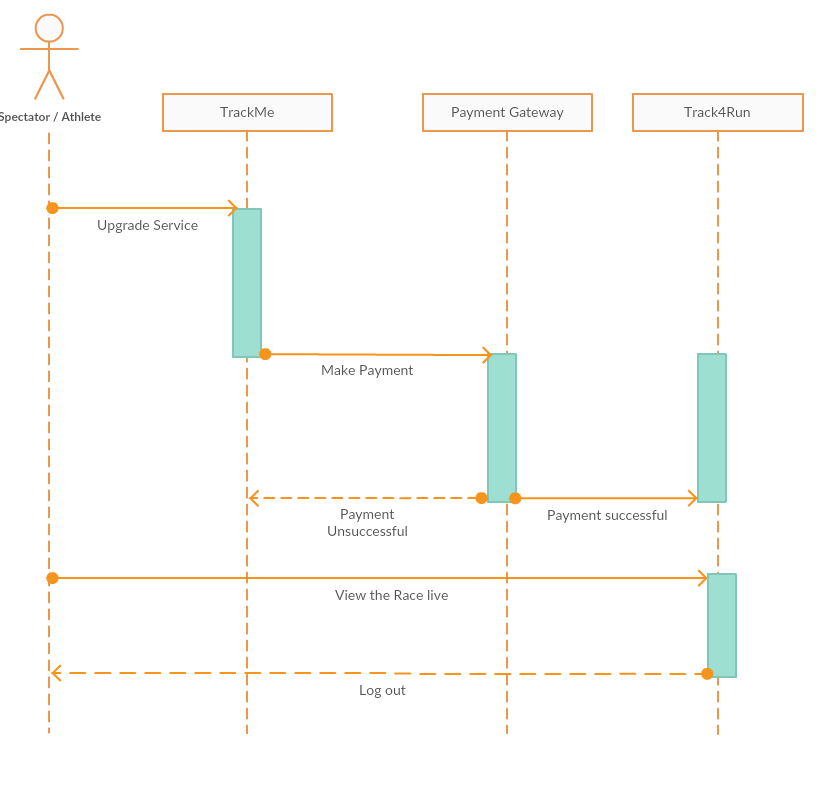
\includegraphics[width=\textwidth]{./RASD_Sequence/7_AthleteSpectator.png}
      	\caption{Athletes participate and Spectators view the race.}
        \label{TrackMe_seq7}
	\end{center}
\end{figure}



\section{Performance Requirements}
\begin{enumerate}
\item The system should at least support 1000 connected users at a time.
\item There is no limit in the number of registered users
\item The push notifications would take around a maximum of 5 seconds.
\end{enumerate}

\section{Design Constraints}
\subsection{Standards Compliance}
\qquad Its users responsibility to ensure that the use of the system complies with the local laws and policies. The system must ask the user for permission to acquire, store and process the personal data and web cookies.

\subsection{Hardware Limitations}
\qquad Only a certain set of wearable devices are supported by our application. 


\section{Software System Attributes}
\subsection{Reliability}
\qquad The system is currently not designed to run in Web Interfaces. The reliability of the system depends on the server.

\subsection{Availability}
\qquad The service shall be continuously available to the user.

\subsection{Security} 
\qquad We ensure the data from the individuals are safe and are only accessible by genuine third party users. 
The requests won’t be accepted unless and until a thorough check of the reasons provided by the 3rd party users or an acceptance from the individual is received. We make sure that third party won’t be able to access any sort of data upon continuous rejection of data requests by individuals. Users banking details are secured through payment via paypal gateway, hence providing a secure transaction. We also use  push messages and thereby enabling the feature of sending encrypted messages rather than the normal notifications which can be accessed with the READ\_SMS permissions.

\subsection{Maintainability}
\qquad The code should be well documented for the future reference for developers. The software development should follow an Object Oriented Model-View-Controller pattern. We will also be automating the testing phase.

\subsection{Portability}
\qquad The software will run on any platform that supports JVM. Currently the application is only available for Mobile applications.The mobile application will be supported by the latest versions of Android and iOS.

%%%%%% ALLOY %%%%%%%%
\chapter{Alloy Model}
\label{ch:alloy}
\subsection{Description}
To execute the main objective, the alloy model depicts the following logics:
\begin{itemize}
\item There are two users individual and third party.
\item Individual has one wearable device that gives Location and Health vitals of that Individual.
\item Third Party can make Group Request and Individual Request.
\item When the health status of an Individual is below the threshold value, the critical condition is True.
\item The ambulance gets the details of the individual whose critical condition is true.
\item The details of the individual is connected to the ambulance that is near to the individual location.
\item An organizer is a Third Party who organizes the Event.
\item An Athlete is an Individual who joins the Event.
\item A spectator can be both Individual and Third party who watches the event.
\item An event has date, time, and location.
\end{itemize}
\subsection{Alloy code}
\begin{figure}[H]
	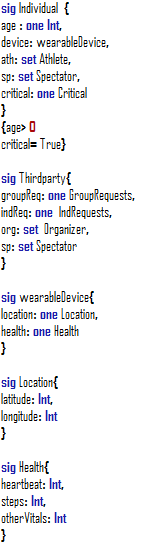
\includegraphics[width=5cm,height=18cm]{./Alloy/sig1.PNG}
\end{figure}
\begin{figure}[H]	\includegraphics[width=5cm,height=18cm]{./Alloy/sig2.PNG}
\end{figure}
\begin{figure}[H]	\includegraphics[width=\linewidth]{./Alloy/sig3+fact1.PNG}
\end{figure}
\begin{figure}[H]	\includegraphics[width=16cm,height=18cm]{./Alloy/fact2+assert1.PNG}
\end{figure}
\begin{figure}[H]	\includegraphics[width=16cm,height=12cm]{./Alloy/assert2+pred.PNG}
\end{figure}
\subsection{Result}
\begin{figure}[H]	\includegraphics[width=\linewidth]{./Alloy/Result.PNG}
\end{figure}
\subsection{Alloy Model}
\begin{figure}[H]	\includegraphics[width=\linewidth]{./Alloy/Final_model.PNG}
\end{figure}


%%%%%% EFFORT %%%%%%%%
>>>>>>> c41ec8f0b0b1545b1fda6c11f51fbdc5631db9e7
\chapter{Effort}
\label{ch:effort}

<<<<<<< HEAD
Hours of Work
\subsection{Haritha Harikumar}
\begin{table}[H]
	\centering
    \begin{tabular}{|l|l|l|}
    \hline
     \textbf{Date} & \textbf{Task} &\textbf{ Hours}\\
    \hline
    15/10/2018 & Understanding Project Specifications & 1\\
    \hline
    16/10/2018 & Brainstorming Problem(Group Work) & 0.5\\
    \hline
    18/10/18 & Identifying goals and set deadlines(Group Work) & 2.5\\
    \hline
    20/10/2018 & Goals, Assumptions and Purpose & 2\\
    \hline
    21/10/2018 & Product Functions & 2\\
    \hline
    18/10/18 & Identifying goals and set deadlines(Group Work) & 2.5\\
    \hline
    25/20/2018 & All Diagrams & 2\\
    \hline
    29/10/2018 & Use Case Diagram & 2\\
    \hline
    31/10/2018 & Functional Requirement & 3\\
    \hline
    08/11/18 &	Final Draft of RASD(Group Work) &	2\\
    \hline
    09/11/2018 & State Diagram & 3\\
    \hline
    07/11/2018 & Alloy & 2\\
    \hline
    11/11/2018 & Alloy(Group Work) & 3\\
    \hline
    & \textbf{Total}	& \textbf{36}\\
    \hline
    \end{tabular}
\end{table}

\subsection{Saloni Kyal}
\begin{table}[H]
	\centering
    \begin{tabular}{|l|l|l|}
    \hline
     \textbf{Date} & \textbf{Task} & \textbf{Hours}\\
    \hline
    16/10/18 & Brainstorming Problem(Group Work) & 0.5\\
    \hline
    18/10/18 & Identifying goals and set deadlines(Group Work) & 2.5\\
    \hline
    19/10/18 & Scope, Product Functions and Dependencies & 2\\
    \hline
    20/10/18 & Software Interfaces, Definitions and Acronyms & 1\\
    \hline
22/10/18 & Discuss rest plan(Group Work) & 3\\
\hline
30/10/18 & All Diagrams Discussion(Group Work) & 2\\
\hline
31/10/18 & All Diagrams Discussion(Group Work) & 2\\
\hline
02/11/18 & Initiate Alloy(Group Work) & 1\\
\hline
03/11/18 & Alloy(Group Work) & 3\\
\hline
05/11/18 & User Interface: Mock-ups & 4\\
\hline
06/11/18 & User Interface: Mock-ups & 2\\
\hline
06/11/18 & Class Diagram & 1\\
\hline
07/11/18 &	Use Case- Automated SOS and tables & 2\\
\hline
08/11/18 &	Final Draft of RASD(Group Work) &	2\\
\hline
09/11/18 &	Sequence Diagram- Draft &	1\\
\hline
10/11/18 &	Alloy(Group Work) &	1\\
\hline
11/11/18 &	Alloy(Group Work) &	3\\
\hline
11/11/18 &	Alloy &	3\\
\hline
	& \textbf{Total}	& \textbf{36}\\  
 \hline
    \end{tabular}
\end{table}

\subsection{Mohini Gupta}
\begin{table}[H]
	\centering
    \begin{tabular}{|l|l|l|}
    \hline
     \textbf{Date} & \textbf{Task} & \textbf{Hours}\\
    \hline
    16/10/18 &	Brainstorming Problem(Group Work) &	0.5\\
\hline
18/10/18 &	Identifying goals and set deadlines(Group Work) &	2.5\\
\hline
19/10/18 &	Goals, Product Functions and Constraints &	2\\
\hline
21/10/18 &	Software Interfaces &	1\\
\hline
22/10/18 &	Discuss rest plan(Group Work) &	3\\
\hline
27/10/18 &	Functional Requirements &	1\\
\hline
30/10/18 &	All Diagrams Discussion(Group Work) &	2\\
\hline
31/10/18 &	All Diagrams Discussion(Group Work) &	2\\
\hline
02/11/18 &	Initiate Alloy(Group Work) &	1\\
\hline
03/11/18 &	Alloy(Group Work) &	3\\
\hline
05/11/18 &	User Interface: Mock-ups &	3\\
\hline
06/11/18 &	User Interface: Mock-ups &	2\\
\hline
06/11/18 &	Class Diagram &	1\\
\hline
07/11/18 &	Communication Interfaces &	1\\
\hline
08/11/18 &	Final Draft of RASD(Group Work) &	2\\
\hline
09/11/18 &	Sequence Diagrams &	3\\
\hline
10/11/18 &	Alloy(Group Work) &	1\\
\hline
11/11/18 &	Alloy(Group Work) &	3\\
\hline
11/11/18 &	Alloy &	2\\
    \hline
	& \textbf{Total}	& \textbf{36}\\   
    \hline
    \end{tabular}
\end{table}
=======
\section{Hours of Work}
<<<<<<< HEAD
\subsection{Saloni Kyal}
\begin{table}[H]
	\centering
    \begin{tabular}{|l|l|l|}
    \hline
     \textbf{Date} & \textbf{Task} & \textbf{Hours}\\
    \hline
    22-11-18 & Analyze DD Document and Decide Architecture (Group Work) & 3 \\
    \hline
	01-12-18 &  Component Diagram and Runtime View(Group work) &  8\\
    \hline
    02-12-18 &  Deployment and DD Documentation  &  3\\
    \hline
    05-12-18 &  Implementation plan, integration and testing  &  4\\
    \hline
		06-12-18 & Component Diagram documentation(Group work) & 3\\
        \hline
        07-12-18 & Requirement Traceability and Automated Component interface & 1\\
        \hline
		08-12-18 & Documentation and RASD version 2(Group work) & 8\\
    \hline
	& \textbf{Total}	& \textbf{30}\\   
    \hline
    \end{tabular}
\end{table}

\subsection{Mohini Gupta}
\begin{table}[H]
	\centering
    \begin{tabular}{|l|l|l|}
    \hline
     \textbf{Date} & \textbf{Task} & \textbf{Hours}\\
    \hline
    22-11-18 & Analyze DD Document and Decide Architecture (Group Work) & 3 \\
    \hline
	01-12-18 &  Component Diagram and Runtime View(Group work) &  8\\
    \hline
    03-12-18 &  User Interface Design &  4\\
     \hline
        05-12-18 & Requirement Traceability & 1\\
    \hline
		06-12-18 & Component Diagram documentation(Group work) & 3\\
        \hline
		06-12-18 & Documentation & 3\\
        \hline
		08-12-18 & Documentation and RASD version 2(Group work) & 8 \\
    \hline
	& \textbf{Total}	& \textbf{30}\\   
    \hline
    \end{tabular}
\end{table}

\subsection{Haritha Harikumar}
\begin{table}[H]
	\centering
    \begin{tabular}{|l|l|l|}
    \hline
     \textbf{Date} & \textbf{Task} & \textbf{Hours}\\
    \hline
    22-11-18 & Analyze DD Document and Decide Architecture (Group Work) & 3 \\
    \hline
    25-11-18 & Introduction, Scope and Details & 1\\
    \hline
	01-12-18 &  Component Diagram and Runtime View(Group work) &  8\\
    \hline
    03-12-18 & Software Component Diagram Final & 1\\
    \hline
		06-12-18 & Component Diagram documentation(Group work) & 3\\
        \hline
        07-12-18 & Component Interface Diagram & 2\\
        \hline
		08-12-18 & Documentation and RASD version 2(Group work) & 8\\
        \hline
        08-12-18 & System Architecture and other design constraints & 2\\
        \hline
        09-12-18 & Final Draft & 2\\
    \hline
	& \textbf{Total}	& \textbf{30}\\   
    \hline
    \end{tabular}
\end{table}
=======
\subsection{Haritha Harikumar}
\begin{figure}[H]
	\begin{center}
		\includegraphics[width=\textwidth]{./Diagrams/Effort_Haritha.jpg}
	\end{center}
\end{figure}
\subsection{Saloni Kyal}
\begin{figure}[H]
	\begin{center}
		\includegraphics[width=\textwidth]{./Diagrams/Effort_Saloni.PNG}
	\end{center}
\end{figure}
\subsection{Mohini Gupta}
\begin{figure}[H]
	\begin{center}
		\includegraphics[width=\textwidth]{./Diagrams/Effort_Mohini.PNG}
	\end{center}
\end{figure}

>>>>>>> c41ec8f0b0b1545b1fda6c11f51fbdc5631db9e7
>>>>>>> 113baf26200f5cdcd76ad522dfc4e5917a715c40

\chapter{References}
\begin{itemize}
\item Specification Document: "Mandatory Project Assignment AY 2018-2019"
\item Lucid Chart Tutorials 
\item Design Slides
\end{itemize}


%\appendix
%\chapter{Appendix}`'
%\input{appendix.tex}

%\input{bibilography.tex}

\end{document}